% !TEX TS-program = pdflatex
% !TEX encoding = UTF-8 Unicode

%%% DOCUMENT DEFINITIONS
% \documentclass[11pt]{article}	% use larger type; default would be 10pt
\documentclass{scrartcl}
\setkomafont{author}{\scshape}
\usepackage{blindtext}
\usepackage[utf8]{inputenc}	% set input encoding (not needed with XeLaTeX)

%%% PAGE DIMENSIONS
\usepackage{geometry}		% to change the page dimensions
\geometry{a4paper}		% or letterpaper (US) or a5paper or....
\geometry{margin=3cm}		% for example, change the margins to 2 inches all round

%%% PACKAGES
\usepackage{wrapfig}
\usepackage{textcomp}
\usepackage{gensymb}
\usepackage{graphicx} 	% support the \includegraphics command and options
\usepackage{booktabs} 	% for much better looking tables
\usepackage{array} 		% for better arrays (eg matrices) in maths
\usepackage{url}
\usepackage{enumitem}
\usepackage{longtable}
\usepackage[defaultlines=4,all]{nowidow}
\usepackage{multicol}
\usepackage{tcolorbox}

\usepackage{tikz}
\newcommand*\circled[1]{\tikz[baseline=(char.base)]{
        \node[shape=circle,draw,inner sep=2pt] (char) {#1};}}

% Make TOC and URLs clickable
\usepackage[
    colorlinks,
    pdfborder={0 0 0},
    linkcolor=black,
    citecolor=black,
    filecolor=black,
    urlcolor=blue
]{hyperref}

%%% Adjust paragraph indent and spacing
\usepackage{parskip}

%%% HEADERS & FOOTERS
\usepackage{fancyhdr} 		% This should be set AFTER setting up the page geometry
\pagestyle{fancy} 			% options: empty, plain, fancy

%%% More compact item lists
\setlist[itemize]{itemsep=-3pt,topsep=0pt}

%%% TITLE PAGE
\title{
    \vspace*{4cm}
    \huge{ZEKIT} \\
    Assembling Instructions \\
    \vspace*{0.25cm}
    \small{Revision 1.0 EN - 01/09/2021} \\
    \vspace*{0.5cm}
    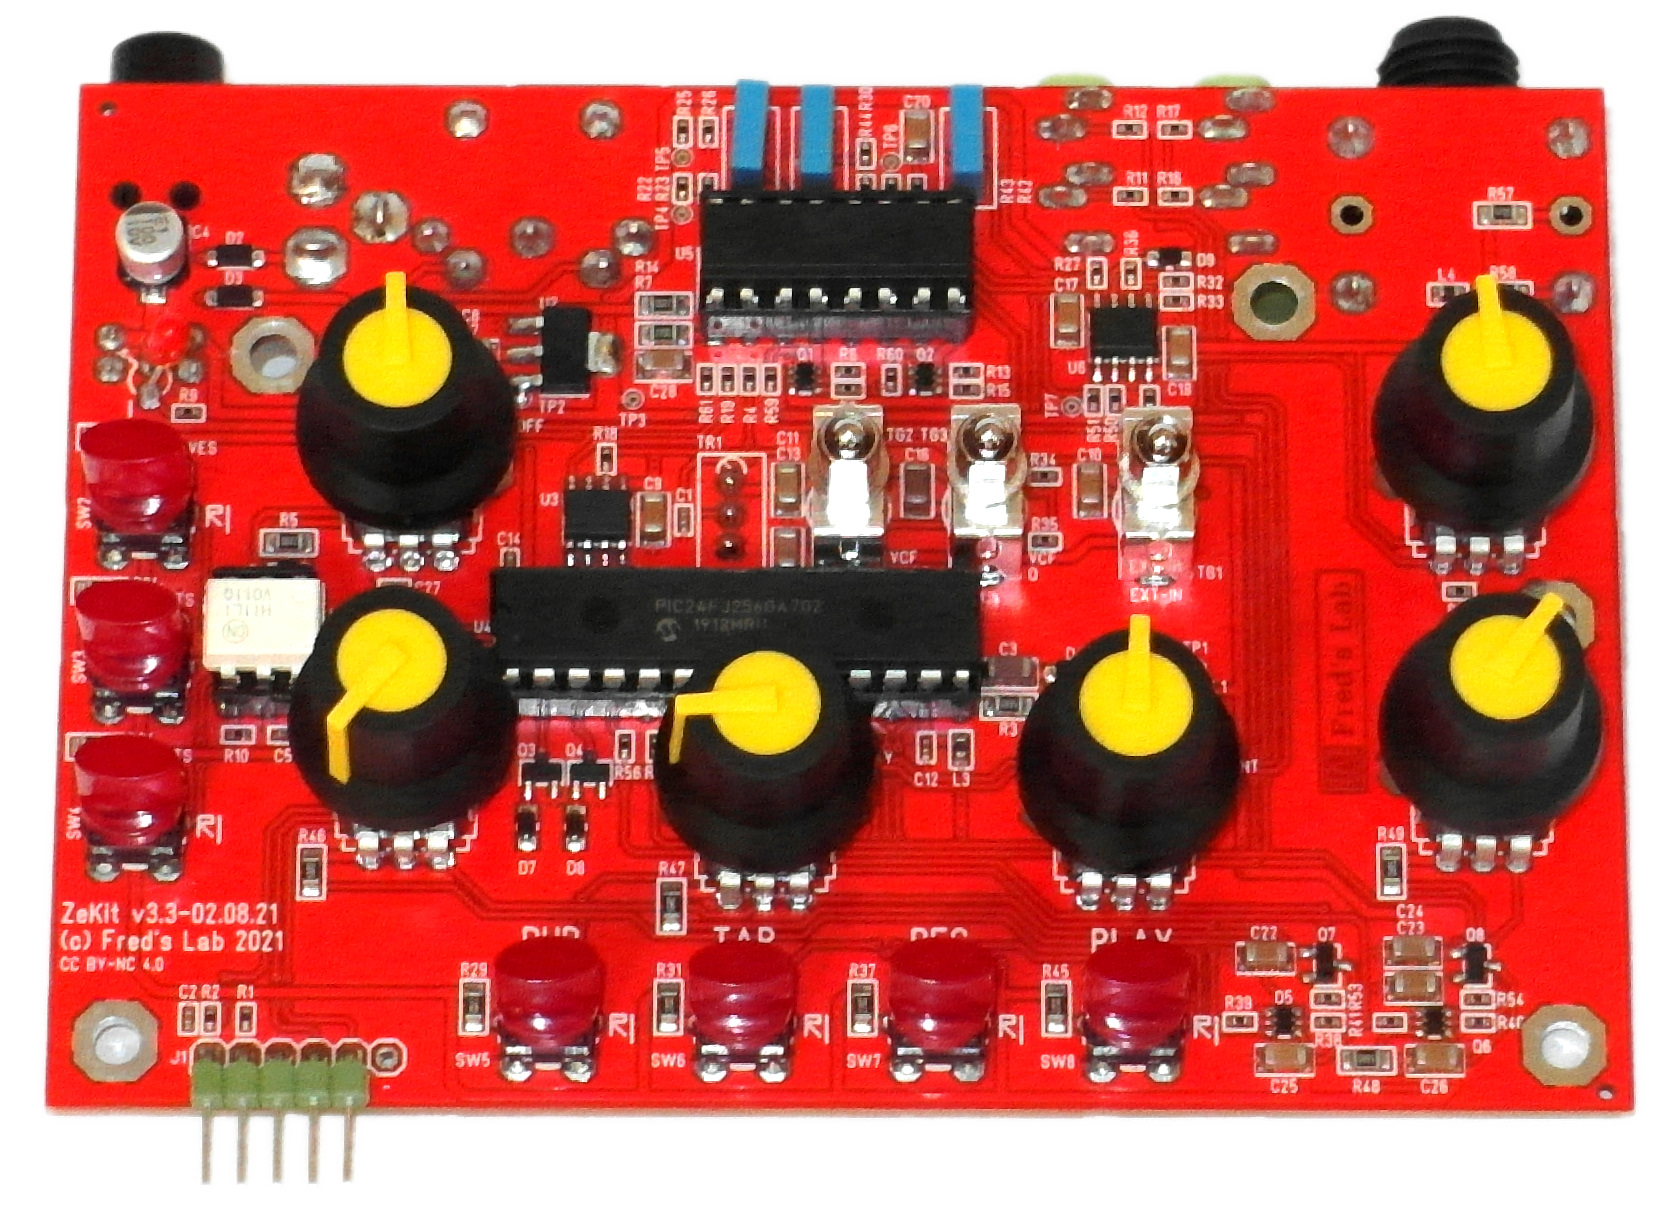
\includegraphics[scale=0.2]{assets/zekit-assembled.jpg}
}
\author{Fred's Lab}

%%% DOCUMENT
\begin{document}

\maketitle

\pagebreak

% ------------------------------------------------------------------------------------------

%%% TABLE OF CONTENTS
\tableofcontents
\pagebreak

% ------------------------------------------------------------------------------------------

\section{Special Thanks}

I would like to thank the following persons for their contributions:

\begin{itemize}
    \item Design consulting: René Schmitz, Oliver Rockstedt
    \item Panel graphics: Serge "erewhon" Beauchamp 
    \item Instruction guide: Oliver Rockstedt, Frédéric Meslin
    \item Beta-testing: Benoit Ruelle, William Zegal, Mathieu Meslin
\end{itemize}

% ------------------------------------------------------------------------------------------

%%% INTRODUCTION
\section{Introduction}

\textbf{Welcome to the ZeKit assembly guide!}

The \textbf{ZeKit} is a fully functionnal 4-voice paraphonic synth kit with \textbf{digital oscillators} and an \textbf{analog filter and amplifier.} It also features two \textbf{analog envelopes} as well as a simple \textbf{pattern sequencer}. The instrument can be controlled via MIDI and handles \textbf{external clock} signals.

Hopefully, you'll learn a lot while building this kit and you'll end up with \textbf{an inexpensive} but \textbf{fun instrument} that will integrate into your studio setup.

\subsection{Required skills}

\begin{itemize}
    \item Basic \textbf{knowledge of synthesis}
    \item Soldering experience with through-hole components
    \item Knowledge on how to interpret a placement diagram
\end{itemize}

\subsection{Required tools}

In order to fully assemble the kit, you'll need the following tools:

\begin{itemize}
    \item A soldering iron with a 3mm flat tip
    \item 1mm solder wire
    \item A wire cutter
    \item A flat head screwdriver
\end{itemize}

\subsection{Required accessories}

\begin{itemize}
    \item Power supply DC 5 to 9V, 0.5A with barrel connector \\
    2.1mm x 5.5mm, center positive (*)
    \item 6.35mm jack audio cable
    \item Optional / Computer, sequencer or MIDI controller
    \item Optional / MIDI cable
\end{itemize}

* A compatible power adapter can be purchased from \textbf{Fred's Lab} website

% ------------------------------------------------------------------------------------------
\pagebreak
\section{Box Content}

In the \textbf{ZeKit} package, you'll find the following components:
\vspace{-0.25cm}

\begin{figure}[!ht]
    \begin{center}
        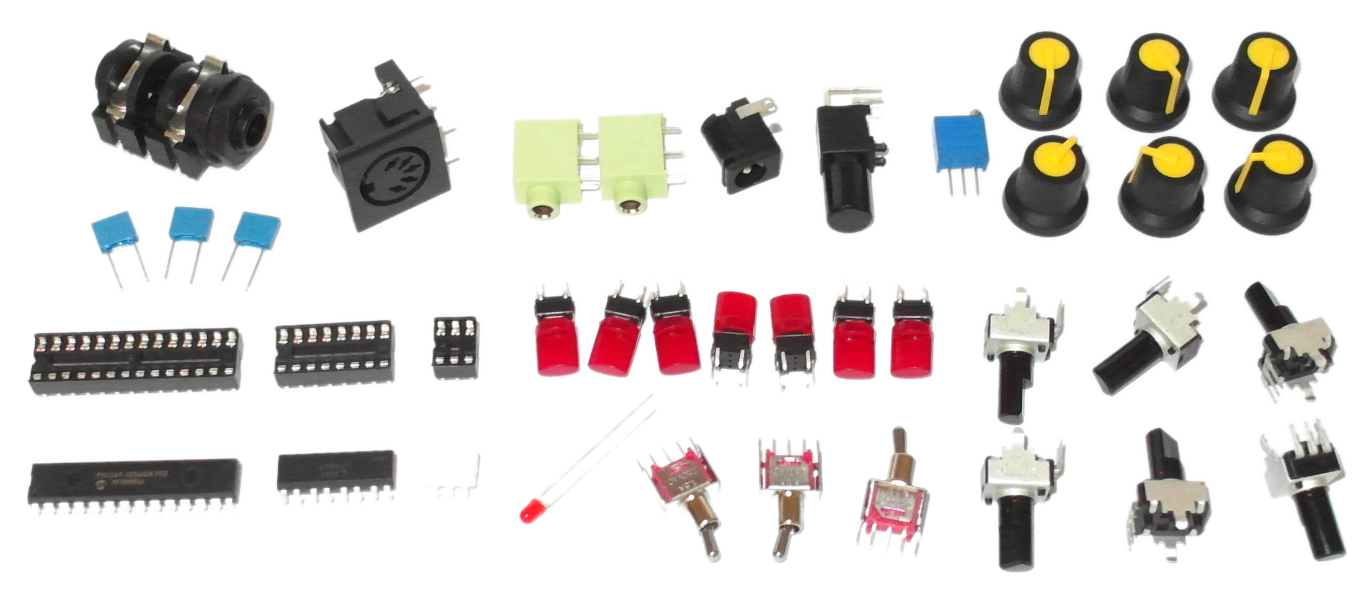
\includegraphics[scale=0.32]{assets/zekit-content.jpg}
        \caption{Components included in the kit}
    \end{center}
\end{figure}

\vspace{0.25cm}

\begin{center}
    \begin{tabular}{|c|l|l|}
        \hline
        \textbf{Amount} & \textbf{Description} & \textbf{Value} \\
        \hline
        1               & Pre-assembled PCB    &                \\
        1               & TRS jack socket      & 6.35mm TRS     \\
        1               & DIN5 socket          &                \\
        2               & TRS jacks socket     & 3.5mm TRS      \\
        1               & Power jack socket    &                \\
        1               & Power switch         &                \\
        1               & Trim potentiometer   & 10k Ohm        \\
        6               & Potentiometer knobs  &                \\
        3               & Film capacitors      & 47nF / 63v     \\
        1               & DIL28 IC socket      &                \\        
        1               & DIL16 IC socket      &                \\
        1               & DIL6 IC socket       &                \\
        7               & Tactile switches     &                \\
        2               & Potentiometers       & 10k Ohm        \\
        4               & Potentiometers       & 100k Ohm       \\
        1               & Microcontroller IC   & PIC24FJ64GA702 \\
        1               & Optocoupler IC       & LTV-847        \\
        1               & Optocoupler IC       & H11L1SM        \\
        1               & LED                  & 3mm red color  \\
        3               & Toggle switches      &                \\
        \hline
    \end{tabular}
\end{center}

\vspace{0.25cm}
Before firing up your soldering iron, \textbf{make sure your kit is complete} and take the time to \textbf{get to know} the different parts.

\pagebreak
\subsection{Pre-Assembled PCB}

The \textbf{ZeKit} makes use of \textbf{SMD} (surface mounted devices) and \textbf{THT} (through hole technology) components. SMD components allow the design to remain \textbf{compact and simple} to manufacture but and more cost effective.

\begin{figure}[!ht]
    \begin{center}
        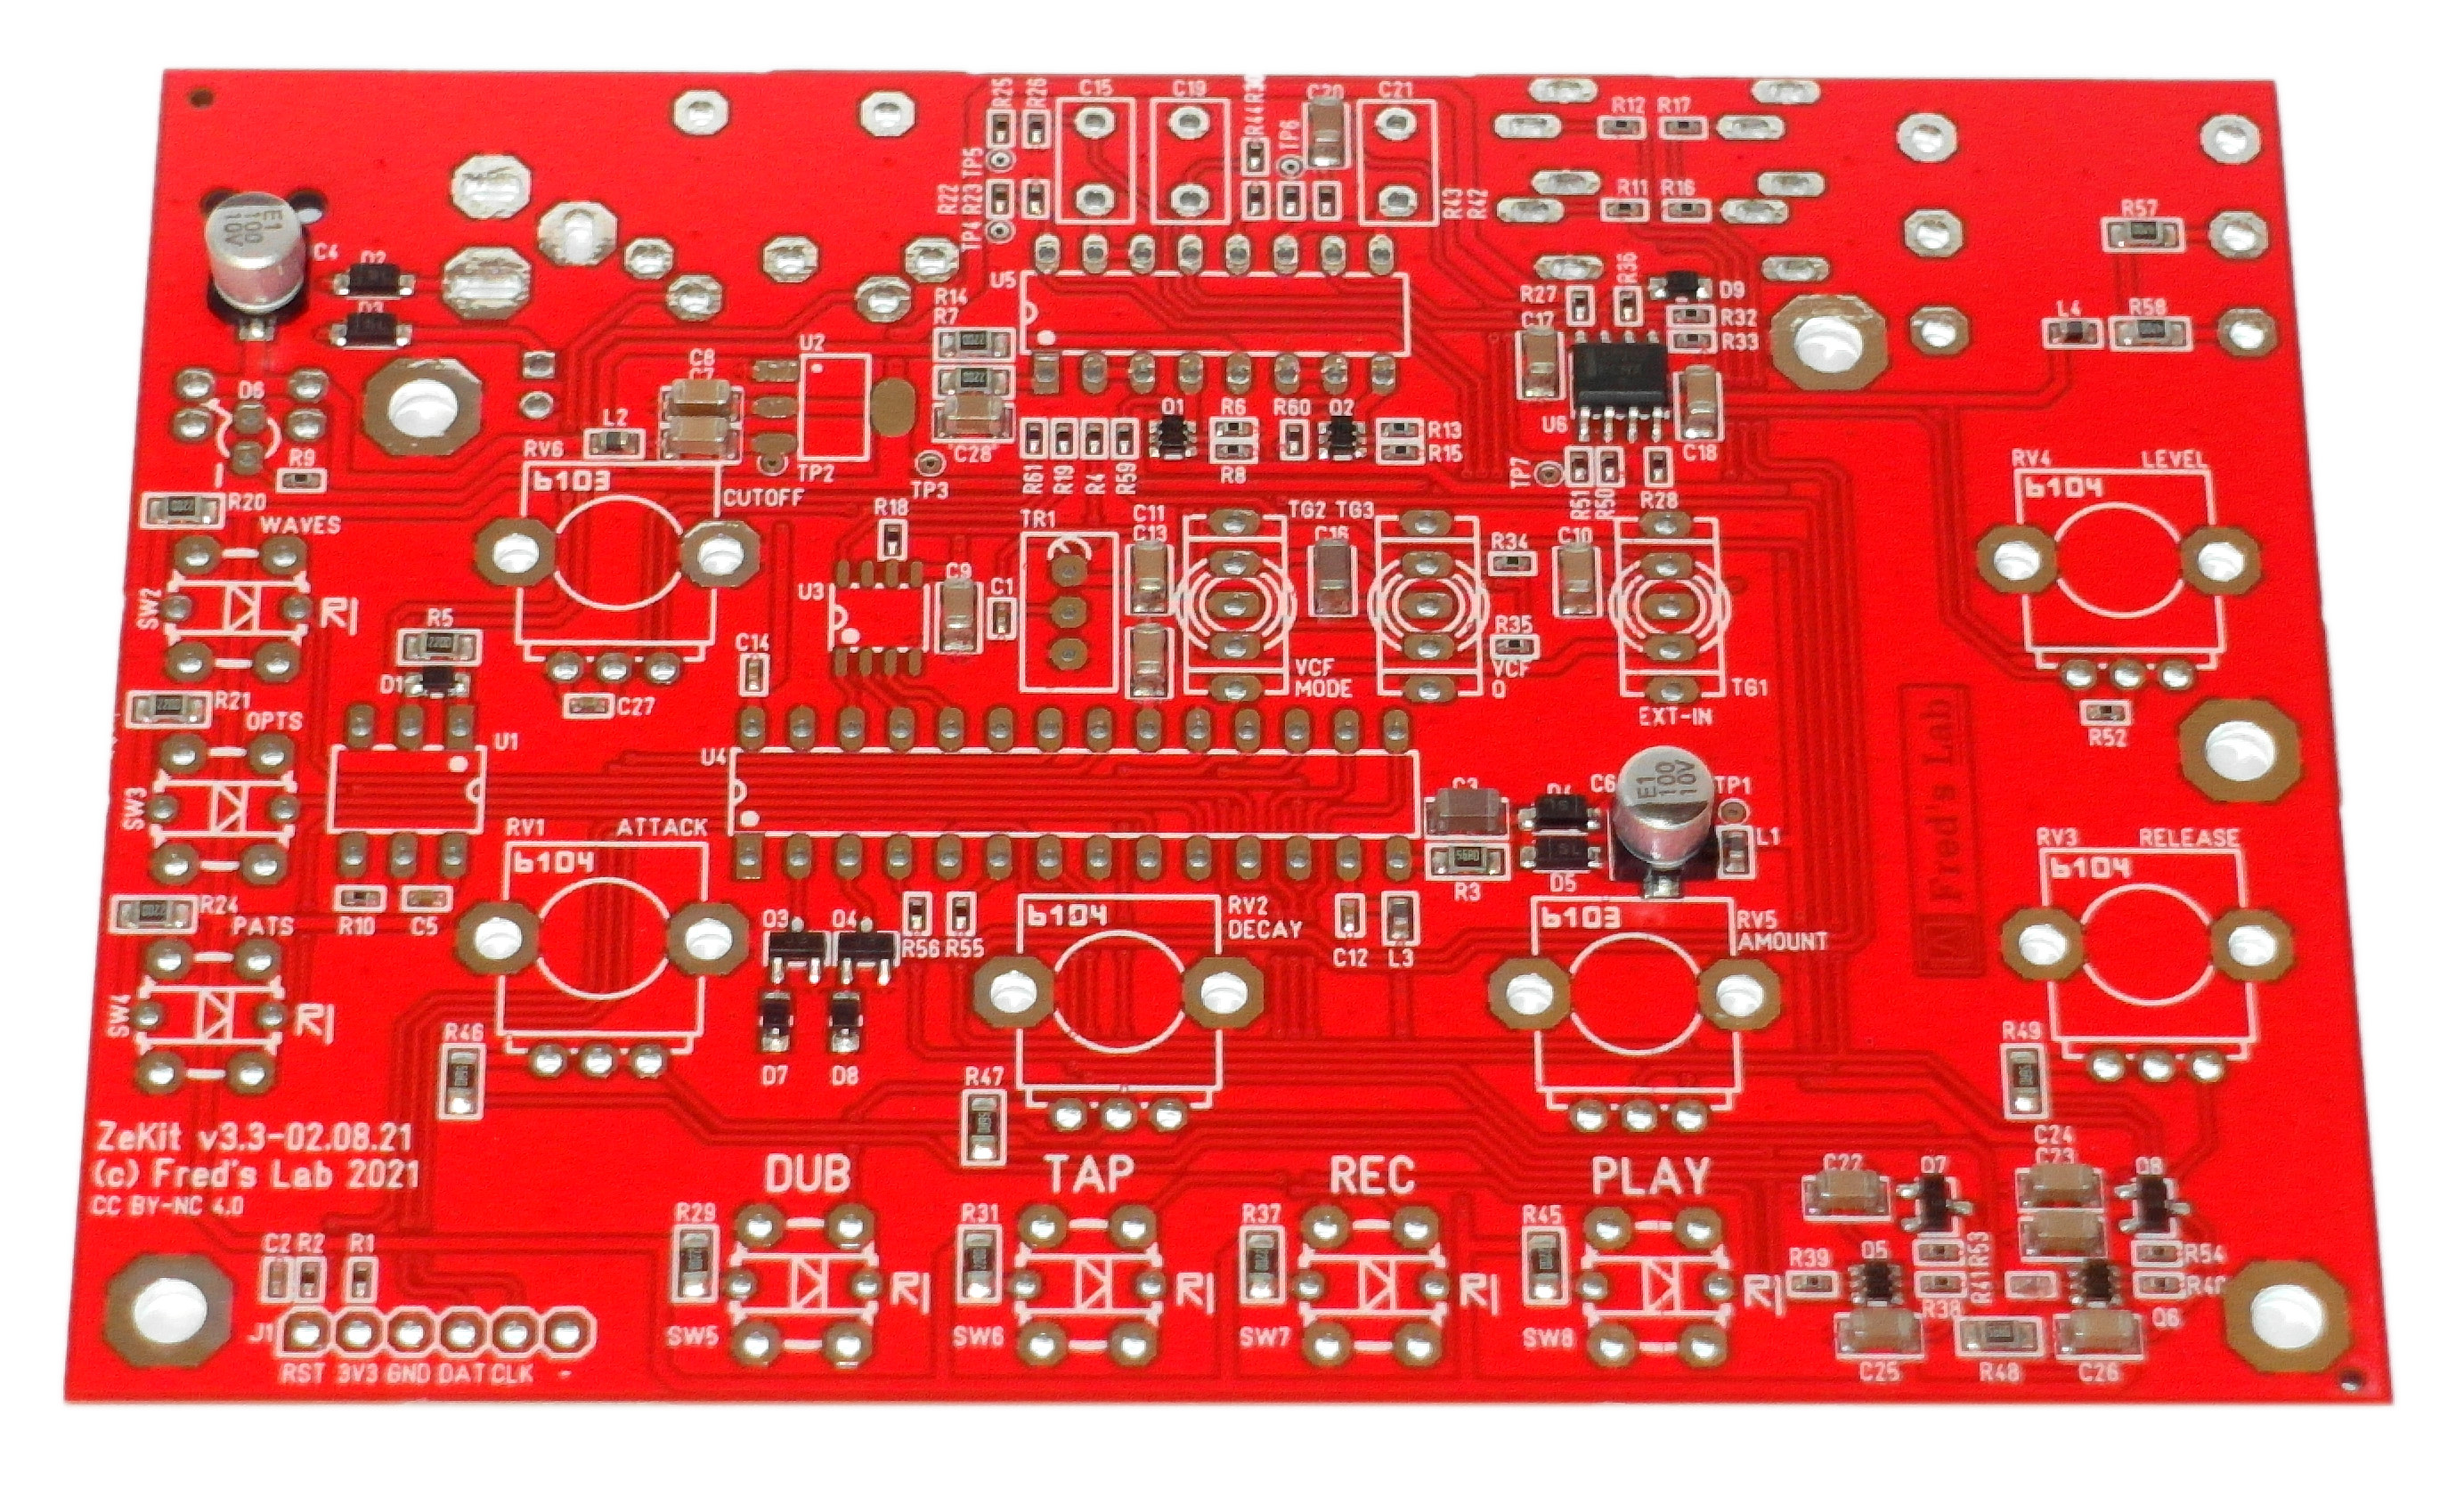
\includegraphics[scale=0.10]{assets/zekit-unassembled.jpg}
        \caption{Pre-assembled ZeKit PCB}
    \end{center}
\end{figure}

All SMD components come already assembled on the PCB (printed circuit board). The THT components are left to be hand soldered, and this is your mission!

\subsection{Provided Parts}

\subsubsection{LED}

\begin{figure}[!ht]
    \begin{center}
        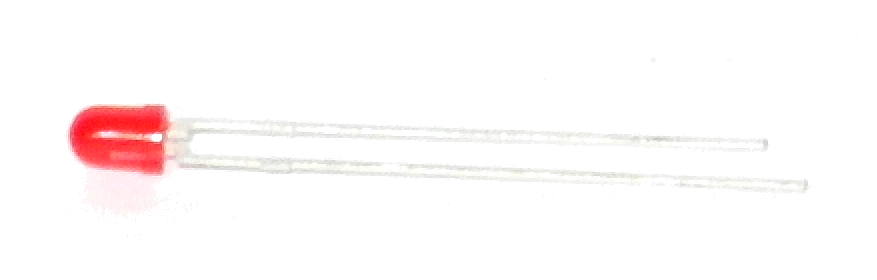
\includegraphics[scale=0.15]{assets/zekit-led.jpg}
        \caption{3mm LED}
    \end{center}
\end{figure}

The \textbf{LED} (Light Emitting Diode) is an indicator that lights up when a current is running through it.
It shows here when the instrument is turned on.

\subsubsection{Tactile Switches}

\begin{figure}[!ht]
    \begin{center}
        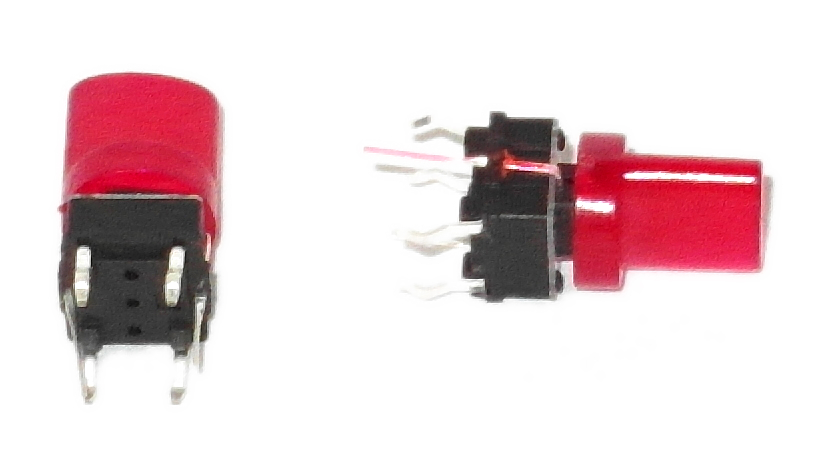
\includegraphics[scale=0.20]{assets/zekit-tacts.jpg}
        \caption{Tactile switches}
    \end{center}
\end{figure}

The \textbf{tactile switches} are \textbf{momentary switches} used as interface buttons.

Their contact is normally open and gets closed when the switch is pressed. These switches have an \textbf{LED built in} that illuminates the cap to show some status information.

They are connected to the microcontroller directly and are used to select the oscillator waveform, choose the sequencer pattern and toggle various options.

\subsubsection{Toggle Switches}

\begin{figure}[!ht]
    \begin{center}
        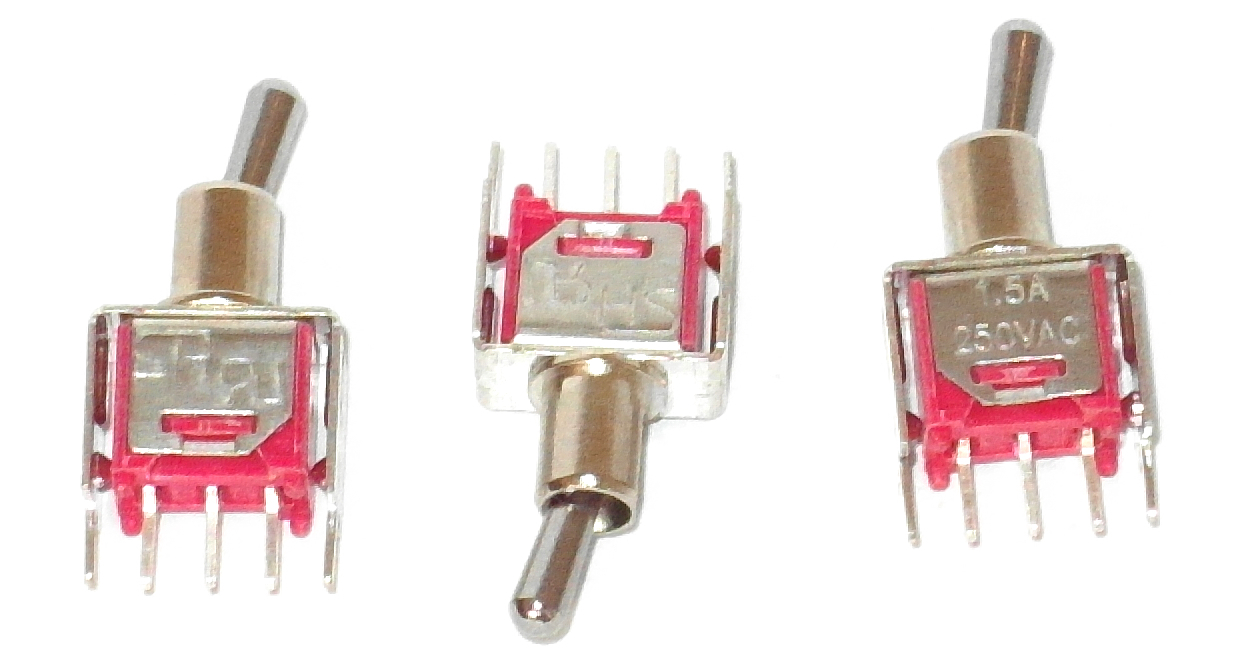
\includegraphics[scale=0.16]{assets/zekit-toggles.jpg}
        \caption{SPDT toggle switches}
    \end{center}
\end{figure}

In contrast to the tactile switches, the \textbf{toggle switches} have \textbf{two stable positions.} They are also called \textbf{SPDT} (single pole, dual throw) switches.
Depending on the lever position, one contact is closed while the other is open and vice versa.

In the \textbf{ZeKit}, these switches select the filter mode (low-pass or band-pass), the filter resonance amount (low or high) and the routing of the external audio input.

\subsubsection{Potentiometers}

\begin{figure}[!ht]
    \begin{center}
        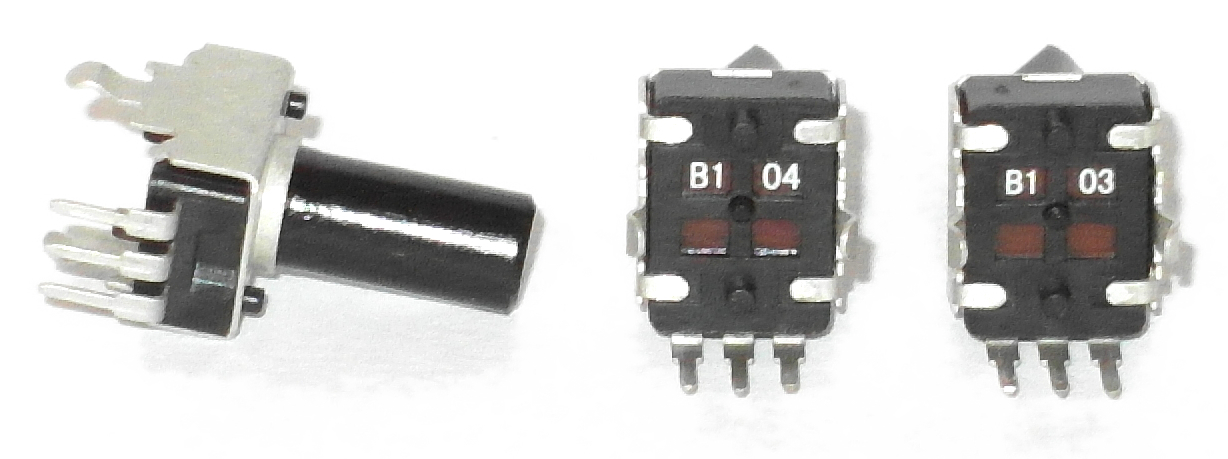
\includegraphics[scale=0.25]{assets/zekit-pots.jpg}
        \caption{Linear mono potentiometers}
    \end{center}
\end{figure}

The \textbf{potentiometers} (or "pots") are \textbf{variable resistors} meant to control sound parameters in the analog domain. They consist of a \textbf{conductive wiper} that slides over a circular \textbf{resistive track} to form a voltage-divider.

The \textbf{ZeKit} uses potentiometers of two different values: \textbf{10k} and \textbf{100k} Ohm.

The pots must not be interchanged or the circuit won't work correctly. They can be easily identified by the label found on their bottom.

$\bullet$ \textbf{B103} = 10k Ohm\\
$\bullet$ \textbf{B104} = 100k Ohm\\

\subsubsection{Trimmer}

\begin{figure}[!ht]
    \begin{center}
        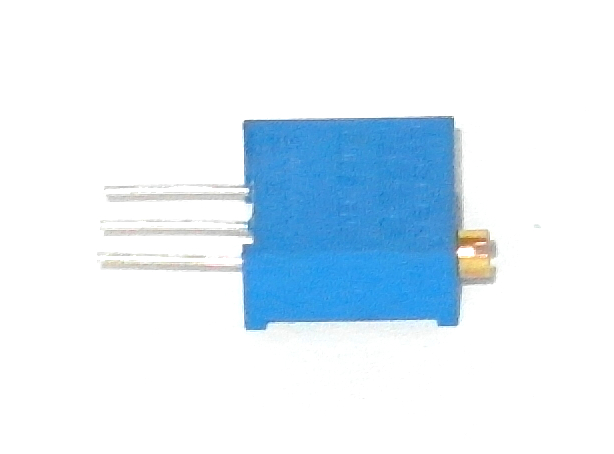
\includegraphics[scale=0.20]{assets/zekit-trimmer.jpg}
        \caption{Multiturn trimmer}
    \end{center}
\end{figure}

\textbf{Trimmers} are specific potentiometers \textbf{intended for calibration}, to compensate for the effects of tolerances in other components manufacturing.

These are smaller than regular potentiometers and need to be adjusted with a flathead screwdriver. They offer a \textbf{great setting precision} since their screw can be turned multiple times. They are also called \textbf{multiturn trimmers}.

The \textbf{ZeKit} uses a single trimmer to define the filter cutoff frequency range.

\subsubsection{Power Switch}

\begin{figure}[!ht]
    \begin{center}
        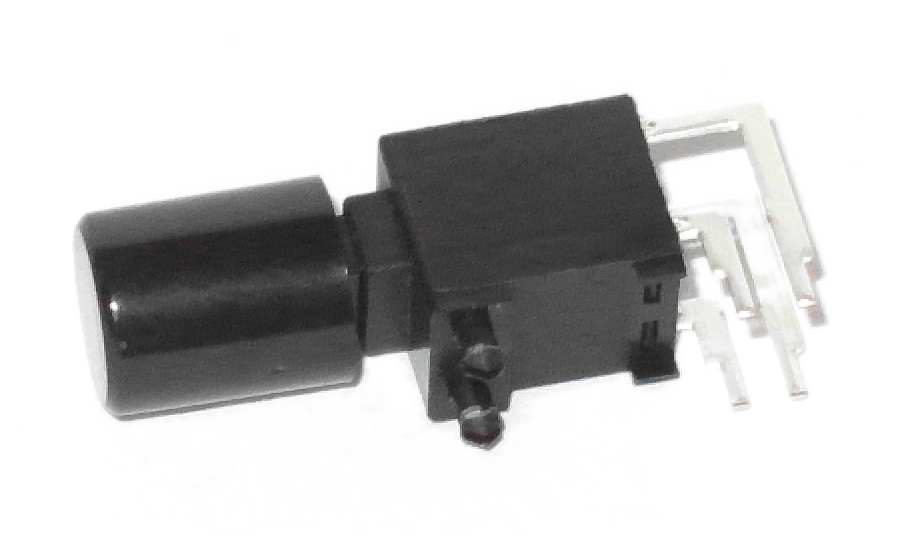
\includegraphics[scale=0.18]{assets/zekit-power.jpg}
        \caption{Power switch}
    \end{center}
\end{figure}

The \textbf{power switch} is a \textbf{latching push button} with a toggle behaviour. \\
Pressed once, the contact closes and remains in this state until it is pressed again. \\
This switch turns the \textbf{ZeKit} power on or off.

\subsubsection{Power Jack Socket}

\begin{figure}[!ht]
    \begin{center}
        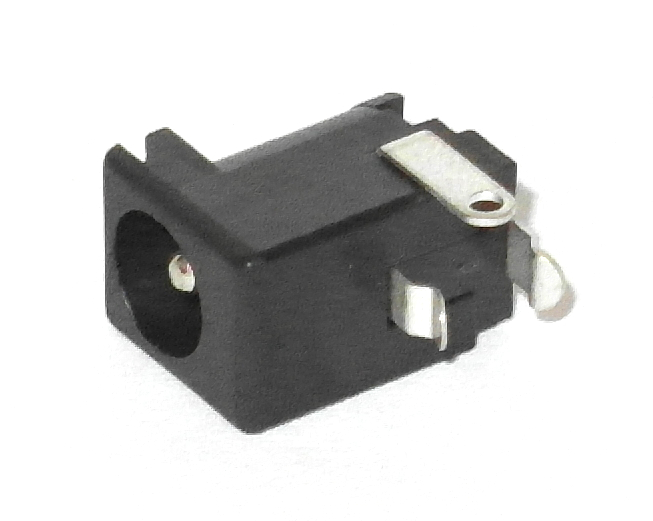
\includegraphics[scale=0.15]{assets/zekit-dcjack.jpg}
        \caption{Power jack socket}
    \end{center}
\end{figure}

The \textbf{power jack} is a standard 2.1mm barrel or coaxial connector that has a widespread use with low voltage power supplies.

The \textbf{ZeKit} can be powered from any DC (direct current) adapter with a voltage ranging from 5V to 9V. The center connection must be positive.

\subsubsection{DIN5 Socket}

\begin{figure}[!ht]
    \begin{center}
        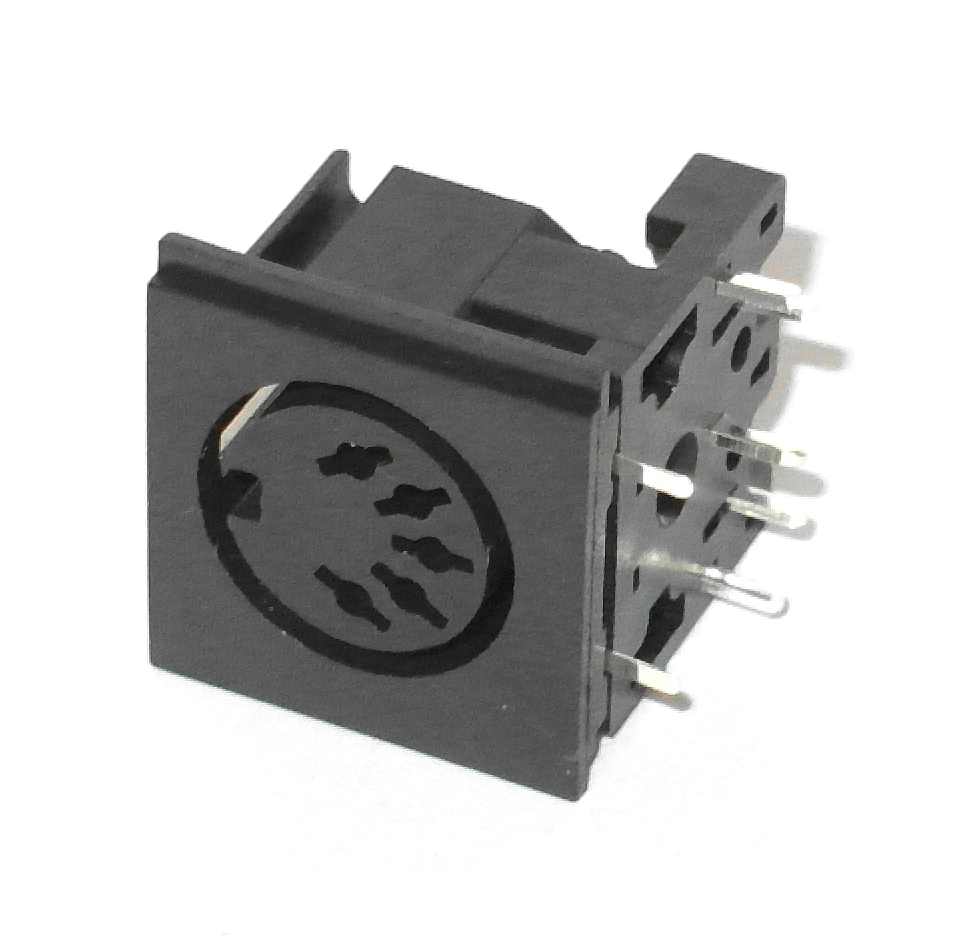
\includegraphics[scale=0.15]{assets/zekit-din.jpg}
        \caption{DIN5 socket}
    \end{center}
\end{figure}

The \textbf{DIN5 socket} is a 5-pin connector used for \textbf{MIDI input}. \textbf{MIDI} stands for \textbf{Music Instrument Digital Interface} and allows the \textbf{ZeKit} to play notes and be synchronized rythmically with other compatible gear, like controllers or sequencers.

\subsubsection{6.35mm TRS Socket}

\begin{figure}[!ht]
    \begin{center}
        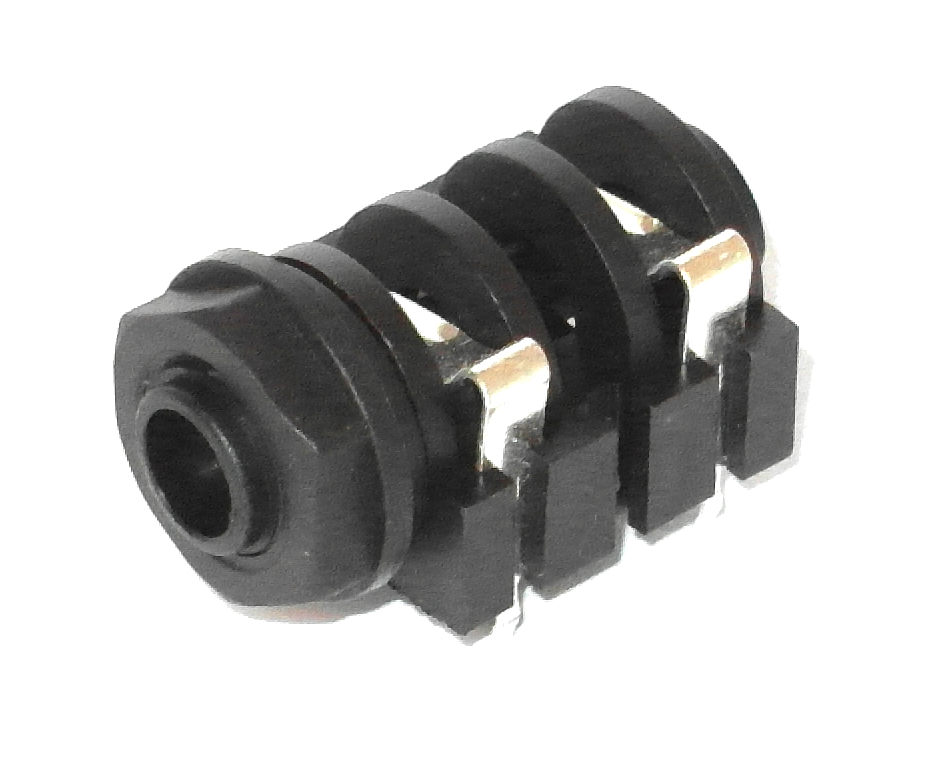
\includegraphics[scale=0.20]{assets/zekit-jack.jpg}
        \caption{6.35mm Jack Socket}
    \end{center}
\end{figure}

The \textbf{TRS jack} stands for "tip, ring and sleeve". This connector is common in \textbf{audio systems} to transmit the sound. The sleeve connection is always grounded whereas the tip and ring respectively carry the left and right audio signals.

This connector is used as the \textbf{ZeKit} line and headphones output.

\pagebreak
\subsubsection{3.5mm TRS Sockets}

\begin{figure}[!ht]
    \begin{center}
        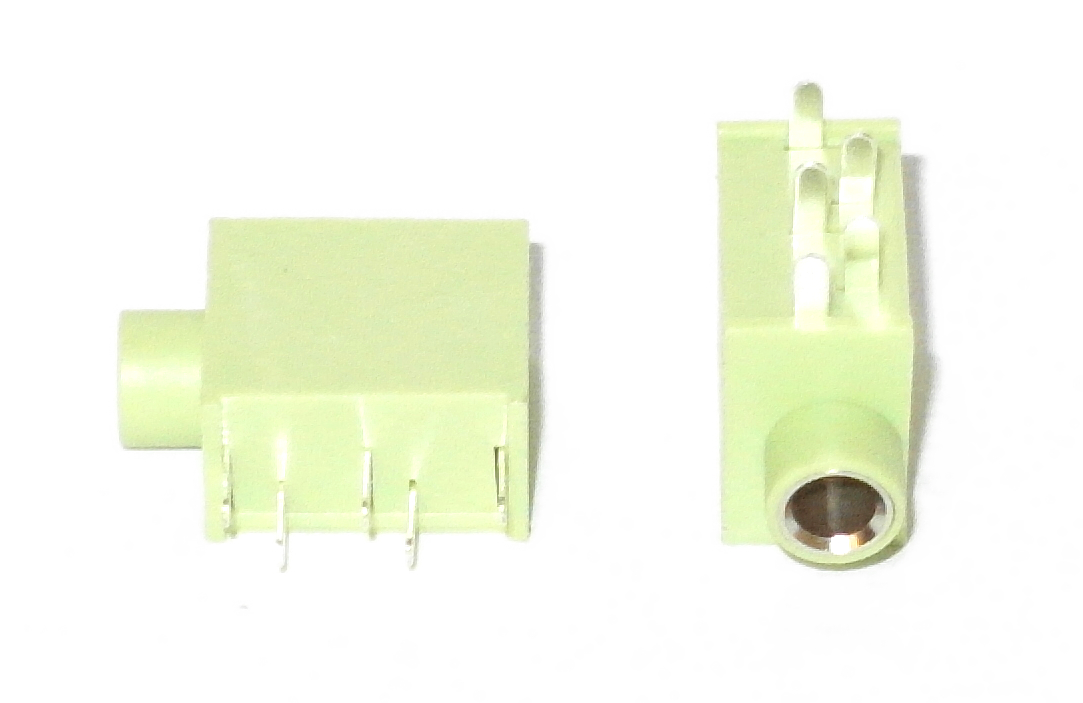
\includegraphics[scale=0.15]{assets/zekit-minijack.jpg}
        \caption{3.5mm Jack Sockets}
    \end{center}
\end{figure}

These sockets are smaller versions of the 6.35mm ones. In the \textbf{ZeKit}, they are used for the \textbf{external audio} and the \textbf{clock or "sync"} inputs.

The \textbf{clock signal} is expected on the jack tip and the sequencer running state (start or stop) on the ring connection. The sleeve connection is grounded.

\subsubsection{Film Capacitors}

\begin{figure}[!ht]
    \begin{center}
        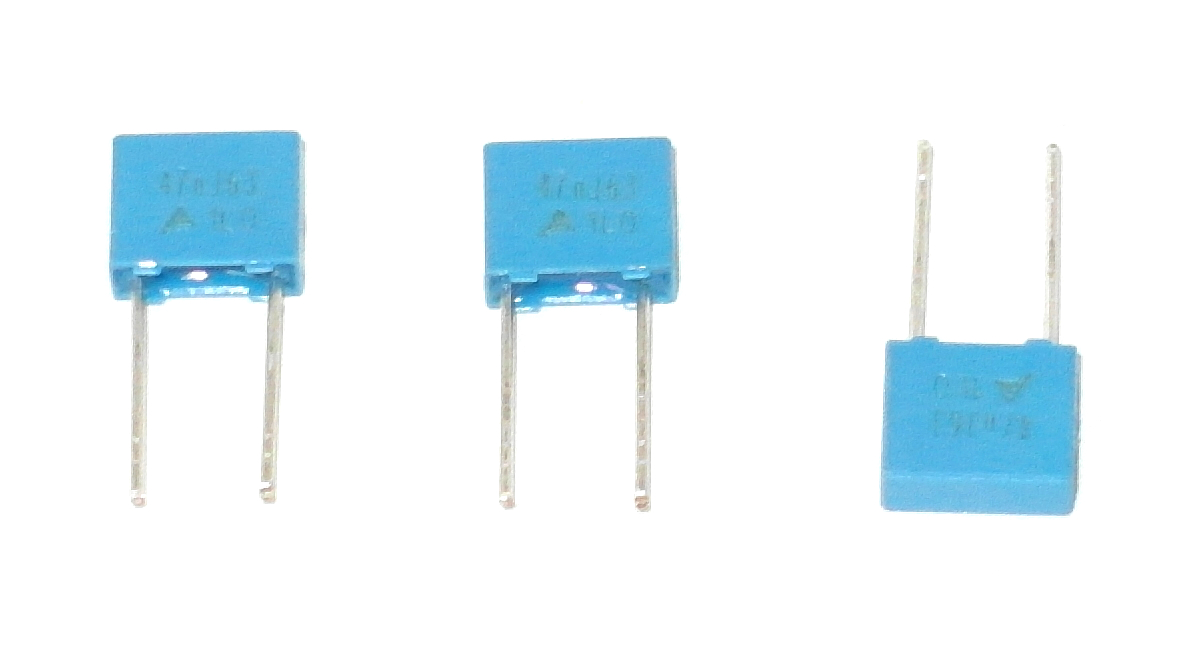
\includegraphics[scale=0.15]{assets/zekit-caps.jpg}
        \caption{47nF Film Capacitors}
    \end{center}
\end{figure}

The \textbf{film capacitors} are capacitors or "caps", they can \textbf{store and release energy.} These types are superior to standard ceramic ones, in terms of \textbf{distortion and noise immunity.}
They also have tighter capacity tolerances.

In the \textbf{ZeKit}, they are used in the voltage controlled filter and amplifier, to process the audio signal.

\pagebreak
\subsubsection{PIC Microcontroller IC}

\begin{figure}[!ht]
    \begin{center}
        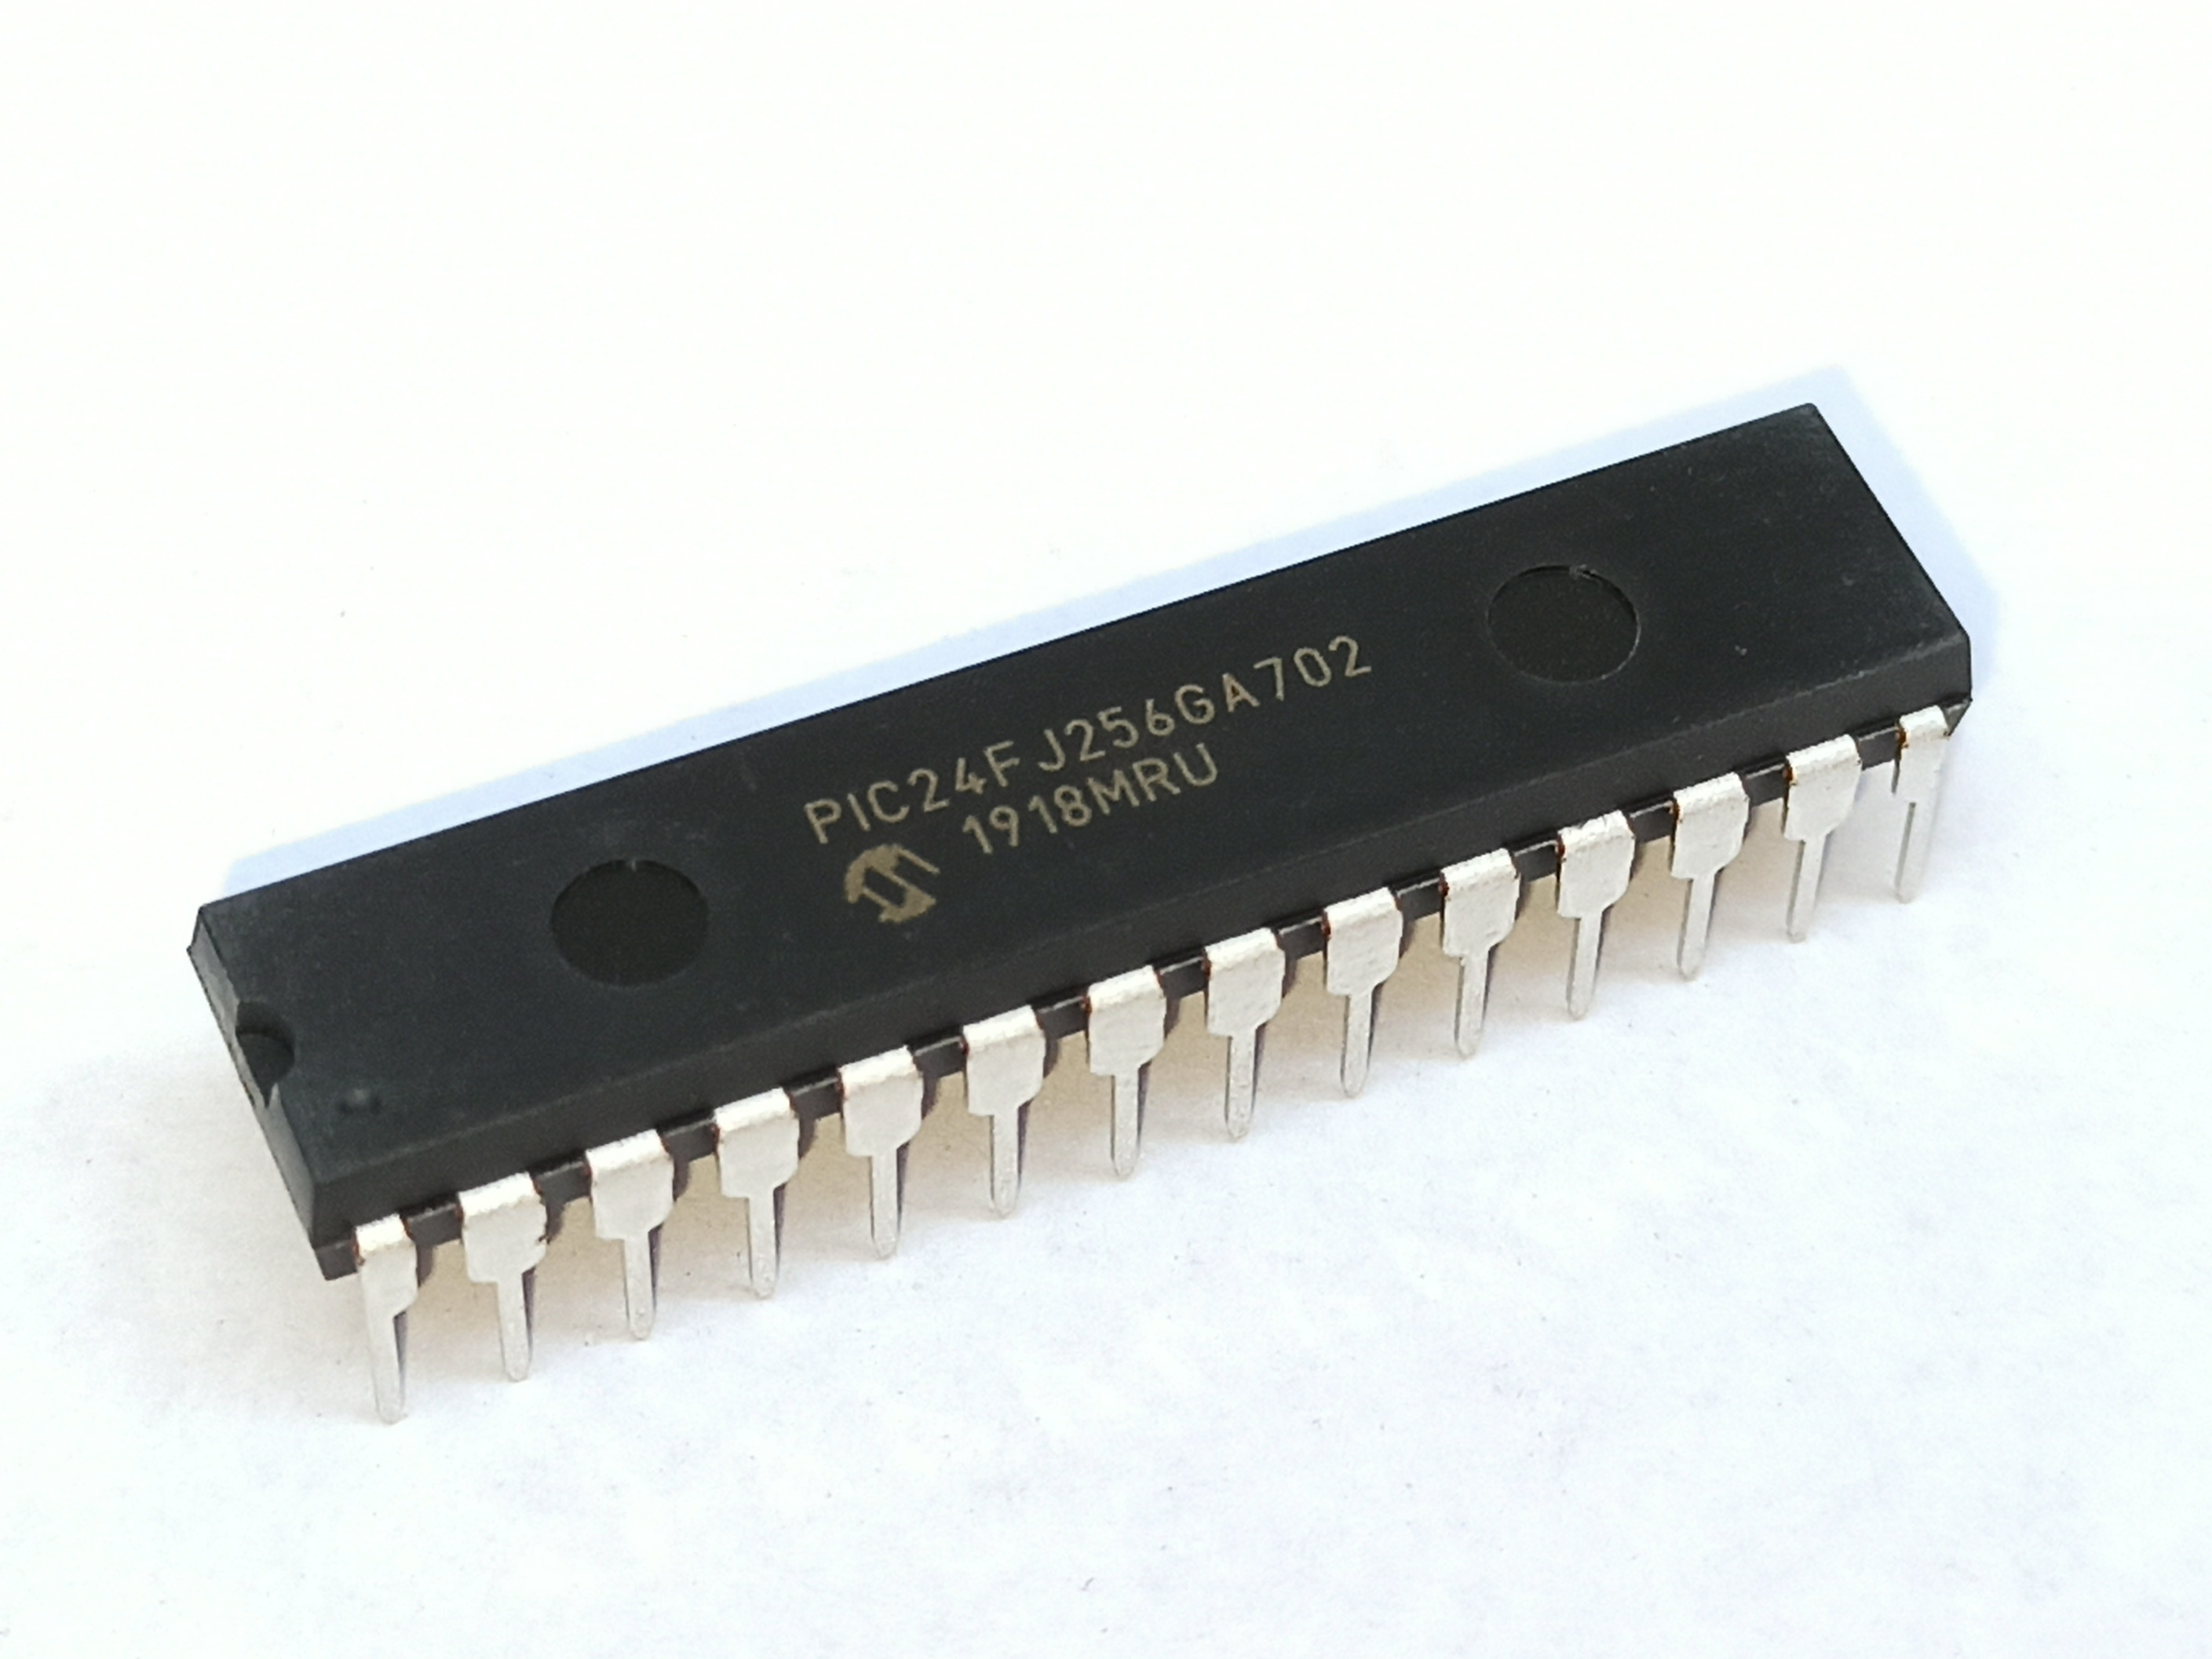
\includegraphics[scale=0.08]{assets/zekit-mcu.jpg}
        \caption{PIC24F 16bit MCU}
    \end{center}
\end{figure}

The \textbf{microcontroller} or "MCU" (Micro-Controller Unit) is an IC (integrated circuit) that contains a \textbf{complete computer.} It features flash memory to store the firmware, RAM to hold data and a processing core with a number of integrated peripherals to communicate with external components.

The \textbf{ZeKit} MCU has a 16bit architecture running at 16Mhz. Its job is to process incoming MIDI messages, handle clock signals, generate the waveforms, run the sequencer, control the envelopes and manage the user interface (buttons and LEDs).
The firmware that handles all these tasks is already pre-programmed by \textbf{Fred’s Lab,} but it can be modified and replaced by the user, using a \textbf{dedicated programmer probe} (non provided).

\subsubsection{Optocoupler ICs}

\begin{figure}[!ht]
    \begin{center}
        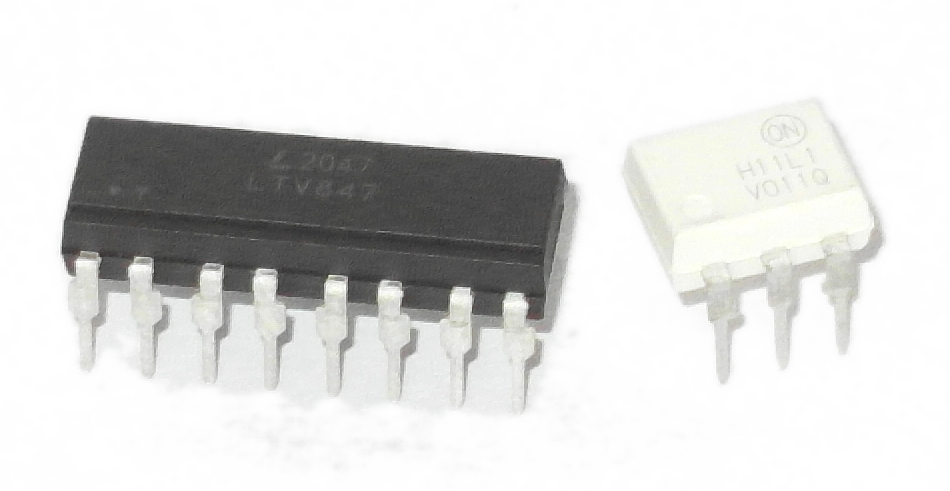
\includegraphics[scale=0.18]{assets/zekit-optocouplers.jpg}
        \caption{Single and quad optocouplers}
    \end{center}
\end{figure}

An \textbf{optocoupler} is a combination of a \textbf{photo transistor} and \textbf{a LED} inside a single package. It is used keep circuits \textbf{electrically isolated} while transferring signals. The conductance of the photo transistor is related to the brightness of the LED.

The \textbf{ZeKit} uses optocouplers for the \textbf{MIDI input} and as \textbf{current controlled resistors} in the VCF (voltage controlled filter) and VCA (voltage controlled amplifier) sections.

\pagebreak
\subsubsection{IC Sockets}

\begin{figure}[!ht]
    \begin{center}
        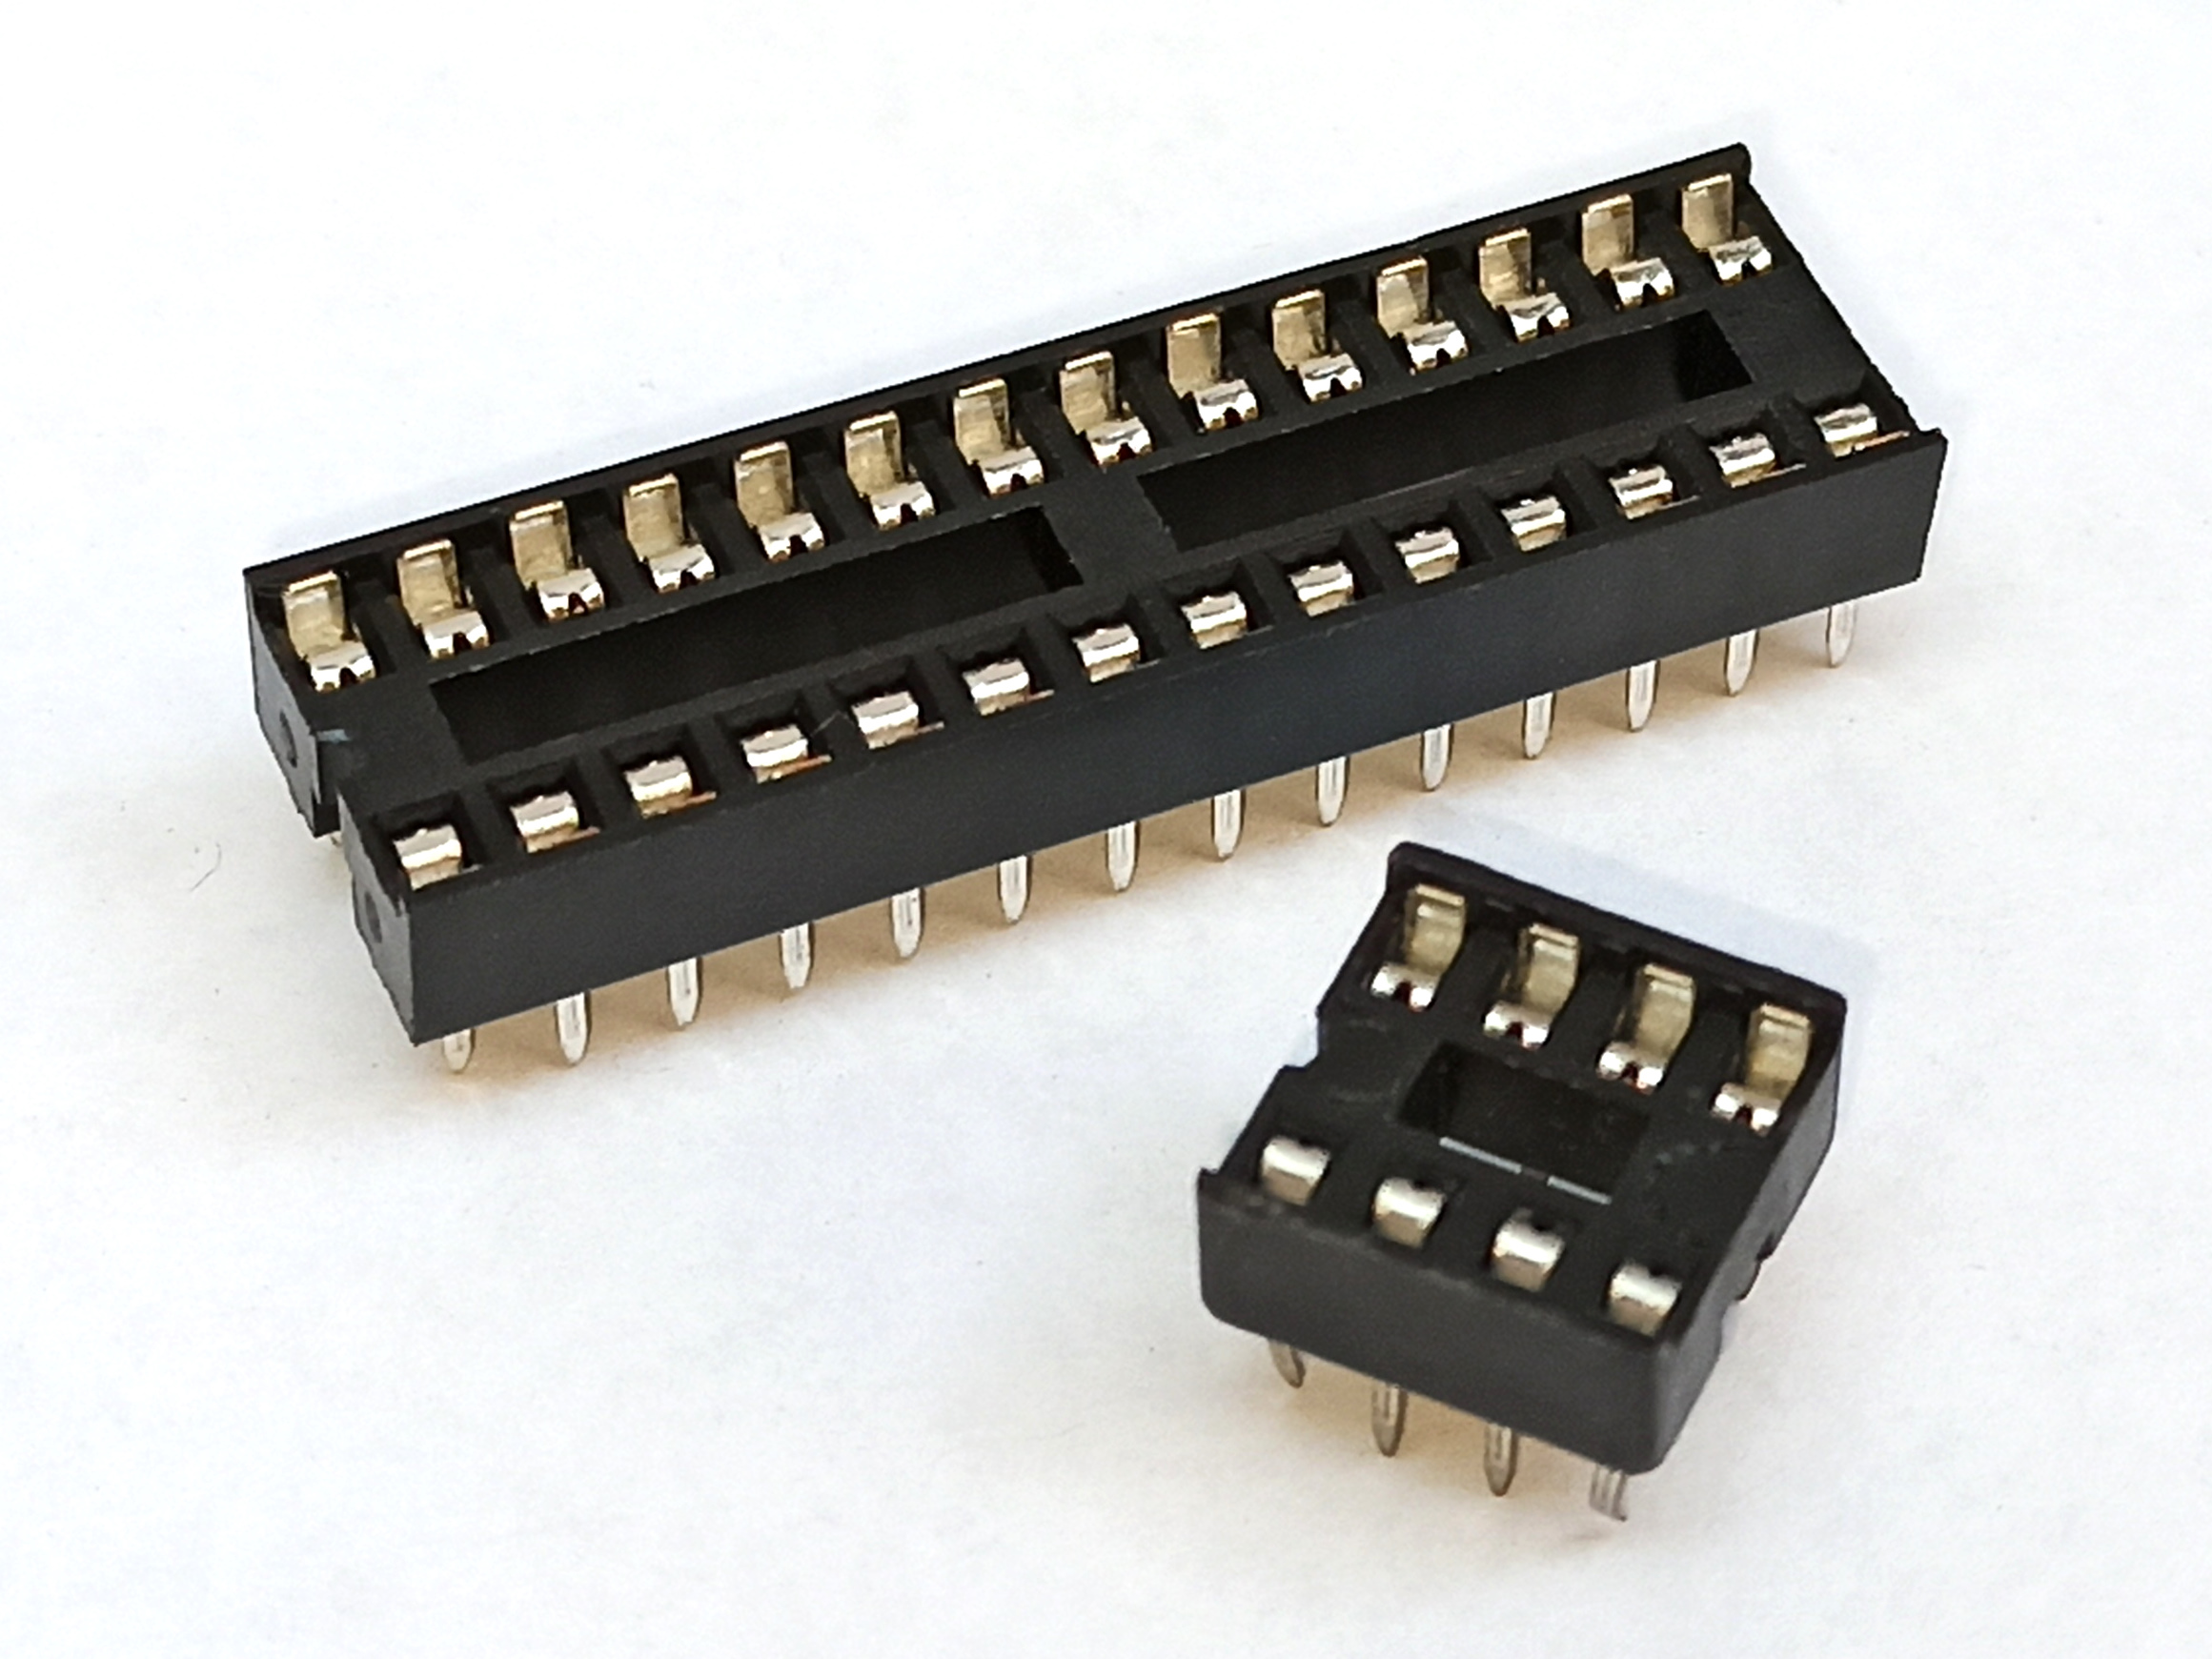
\includegraphics[scale=0.17]{assets/zekit-sockets.jpg}
        \caption{DIP sockets}
    \end{center}
\end{figure}


\textbf{DIP sockets} (Dual In-line Package) are mounted instead of directly soldering the ICs onto the PCB.

While not mandatory, they will protect the ICs from \textbf{overheating} when soldering and keep them \textbf{exchangeable.} Finally, the sockets will prevent the ICs being soldered in "the wrong direction" ... Do not worry, this happens to the best of us!

\subsubsection{Potentiometer Knobs}

\begin{figure}[!ht]
    \begin{center}
        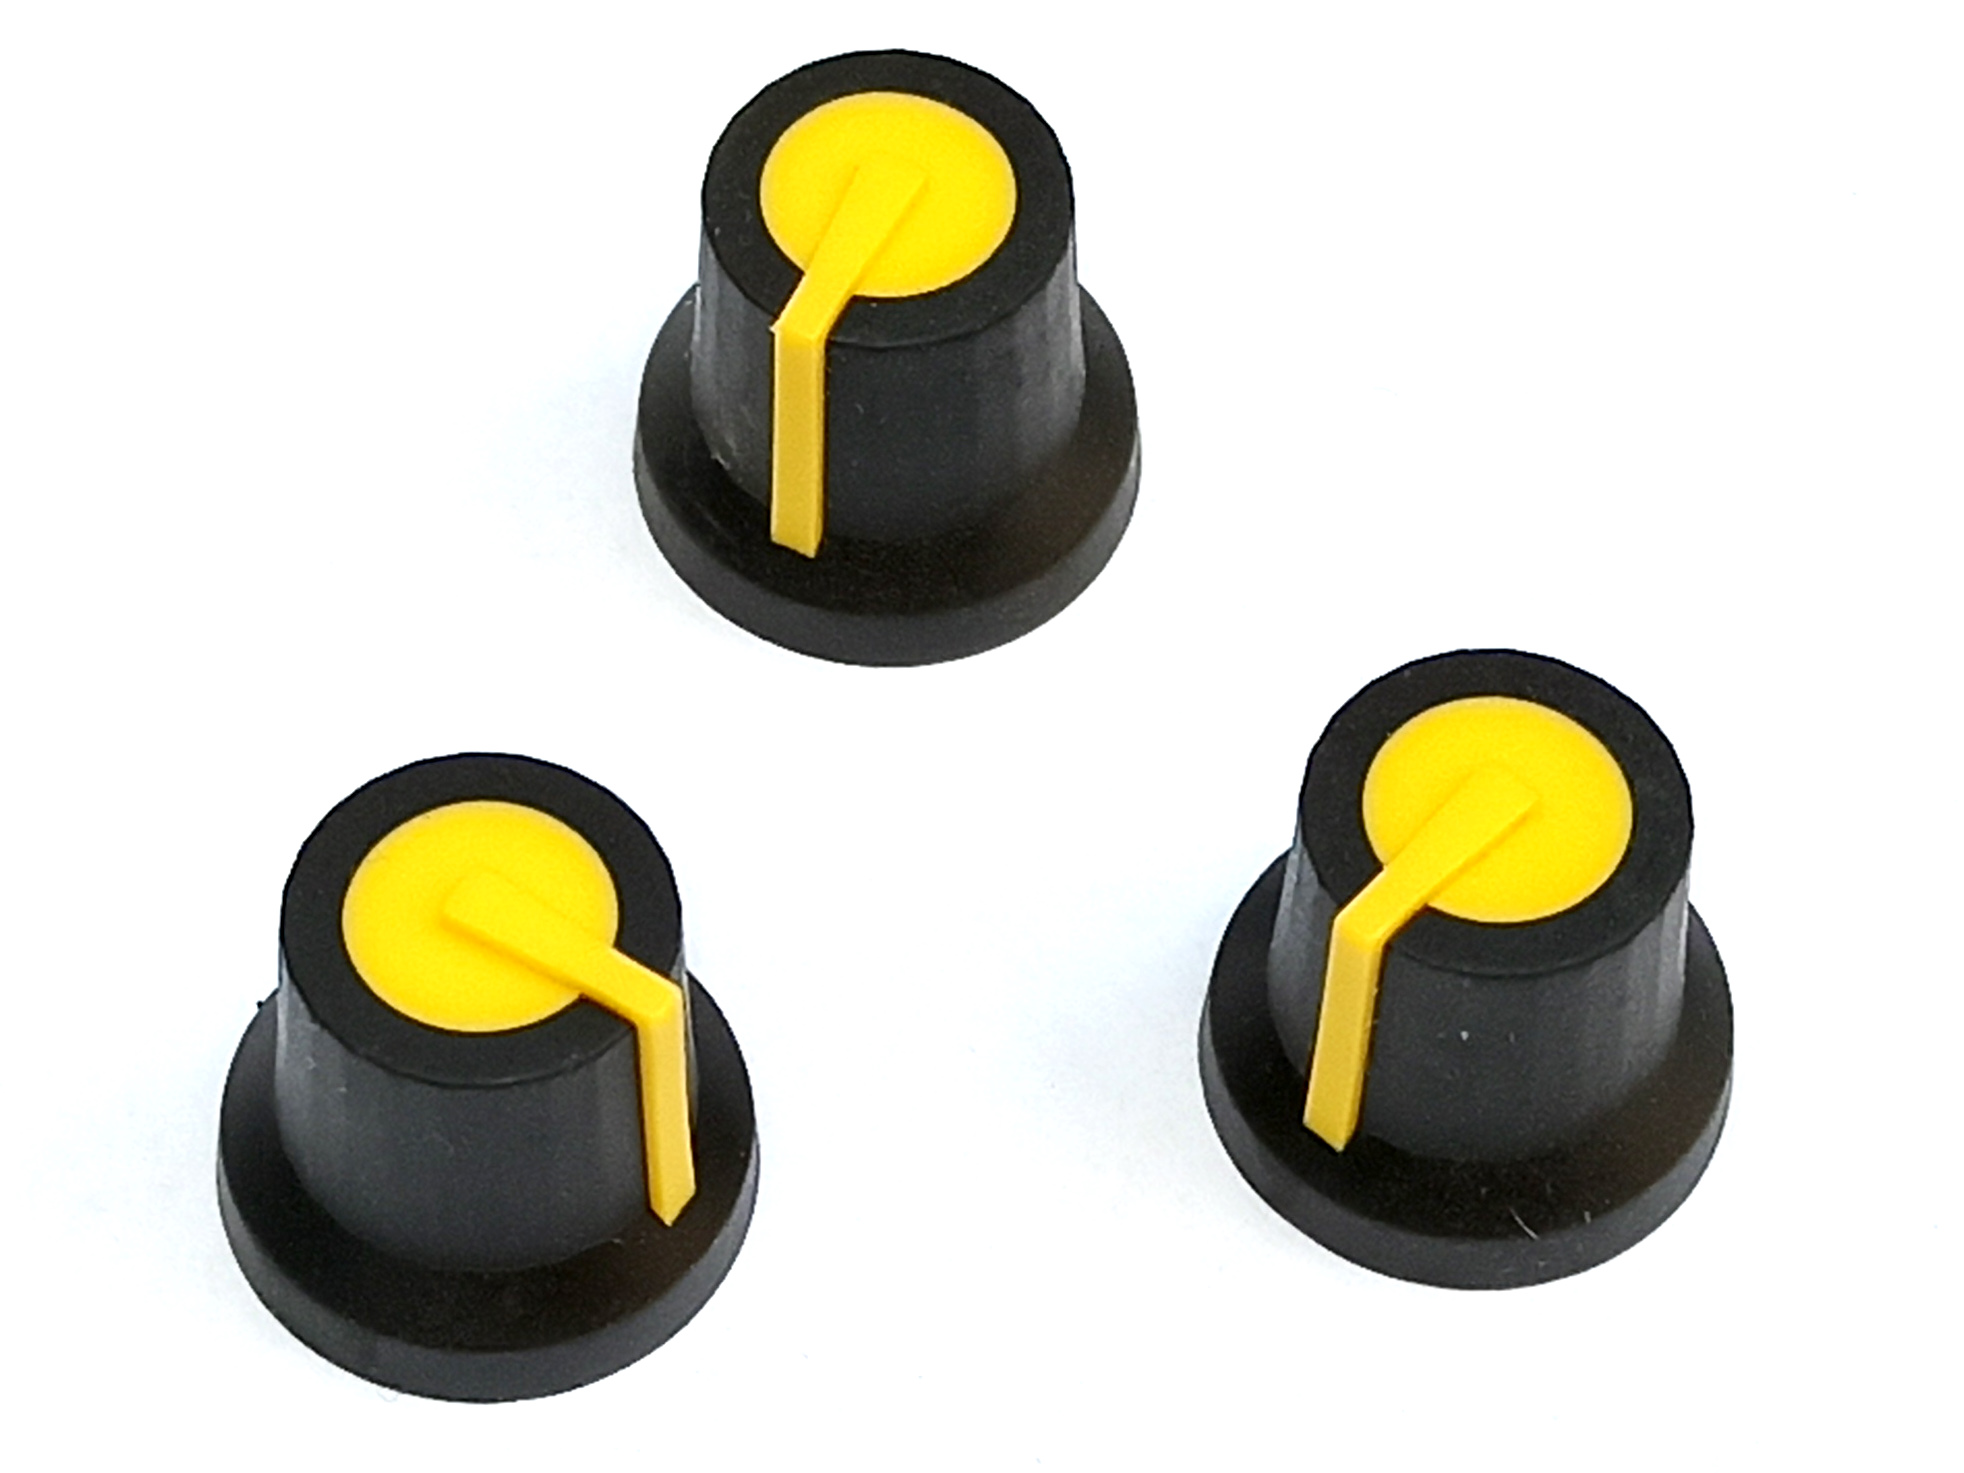
\includegraphics[scale=0.15]{assets/zekit-knobs.jpg}
        \caption{Potentiometer knobs}
    \end{center}
\end{figure}

\textbf{The knobs} are fitted onto the potentiometers after the kit is fully assembled.

They provide the final \textbf{look-and-feel} and allow precise control of the potentiometer and sound settings.

\pagebreak

% ------------------------------------------------------------------------------------------

\section{Assembling the Kit}

\subsection{General Advices}

To maximize your chance of success assembling the \textbf{ZeKit,} work preferably on a tidy \& properly lit surface.
Don't hesitate to use \textbf{magnification} to control your solder joints, reheat with noclean flux if necessary.
Keep unused parts in their original packaging.

Soldering is easier with a \textbf{clean and not oxidized} iron tip. Always switch your iron off when not soldering to extend the tip lifespan!

\subsection{Setting up the soldering gig}

\begin{itemize}
    \item Only work in a well ventilated room
    \item Use SnCuNiGe (SN100C), SN96.5Ag3Cu0.5 (SAC305) or Sn60Pb40
    \item Regularly clean the tip with a wet sponge
    \item Have some duct tape at hand
\end{itemize}

\subsection{How to solder like a Pro}

Great soldering joints can be achieved even with basic equipment and little practice,\\
when respecting the following steps:

\begin{enumerate}
    \item Position (and secure) the component properly
    \item Apply heat to the PCB pad with the iron tip
    \item Bring in the wire until there is enough material
    \item Remove the soldering wire while heating the joint
    \item Pull back the tip from the joint
    \item Let the solder junction cool down naturally
\end{enumerate}

\vspace{0.25cm}
\begin{center}
    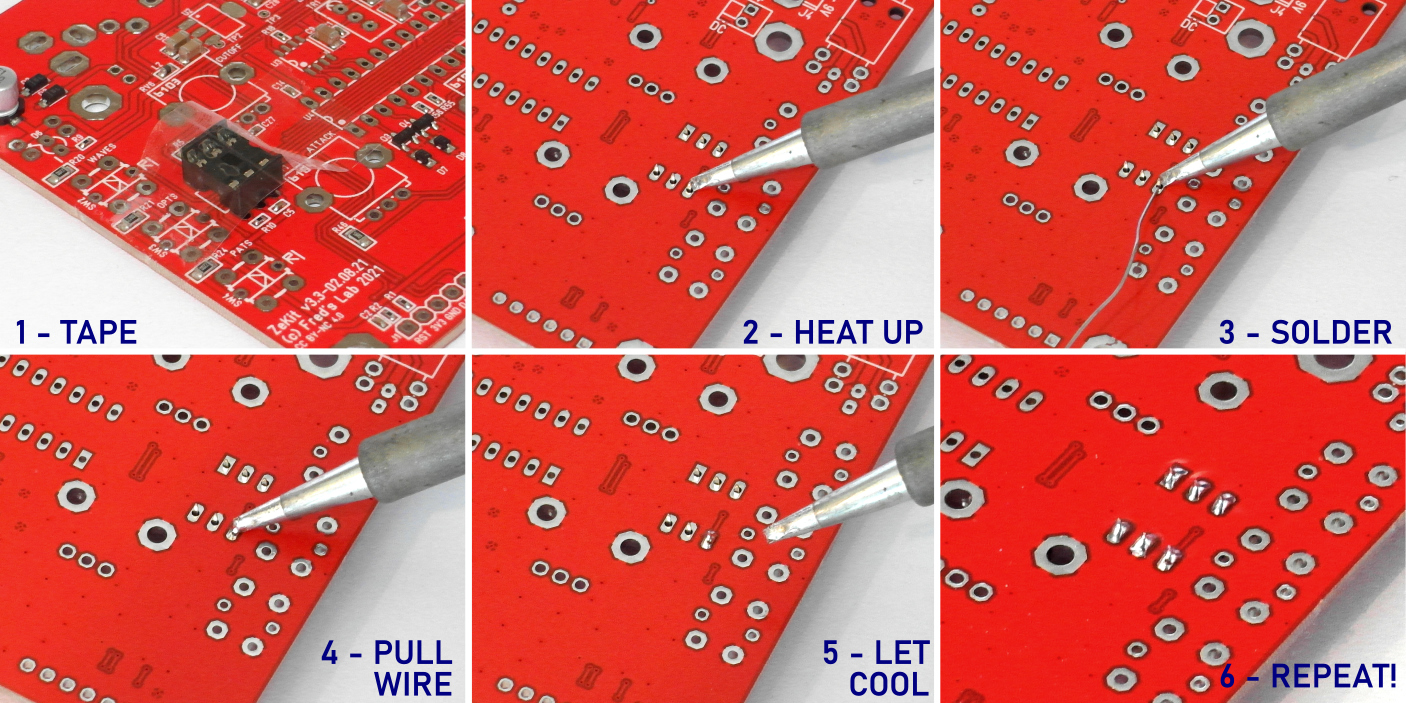
\includegraphics[scale=0.65]{assets/solder-strip.jpg}
\end{center}

\pagebreak
\textbf{Additional Tips:}

\begin{itemize}
    \item Ensure the board is clean before soldering
    \item Use Isopropyl alcohol to clean the PCB (if needed)
    \item Apply noclean flux BEFORE soldering
    \item Double check components orientation
    \item Tape the components before soldering
\end{itemize}

\pagebreak
\subsection{Soldering the Components}

The parts have to be soldered in a \textbf{specific order} that is determined by the placement and size of each component.

Some useful tips:

\begin{itemize}
    \item Tape the components to prevent them from moving or falling off when turning over the PCB for soldering.
    \item All potentiometers, switches and connectors must be \textbf{soldered straight.} \\\\
    Otherwise, the optional panel and housing won't fit. To achieve this, solder only one pin first. Then, correct the component position by \textbf{gently pressing} it in the right position. Finally, solder the remaining pins.
\end{itemize}

\vspace{0.25cm}

\begin{tcolorbox}
    \textcolor{red}{
        \textbf{Some components have a polarity and must be soldered in the right orientation. Even if they fit onto the PCB mechanically in more than one way, using the wrong orientation will result in erroneous operation and can even destroy these parts.}
    }
\end{tcolorbox}

\vspace{0.25cm}

\begin{tcolorbox}
    \textcolor{red}{
        \textbf{All connectors and the power switch are located on the bottom side of the PCB and must be soldered from the top.}
    }
\end{tcolorbox}

\subsubsection{Step 1: IC Sockets}

The IC sockets have a marking on one side. This marking must match the silk screen print of the PCB.

\subsubsection{Step 2: Film Capacitors}

These capacitors are more heat sensitive than other parts. Do not heat the pins for a period longer than 5s. These parts are not polarized and can be soldered in any orientation.

\subsubsection{Step 3: 10k Trimmer}

This trimmer is labeled \textbf{W103}. This part is not polarized and can be soldered in any orientation.

\subsubsection{Step 4: Tactile Switches}

While the switch itself works in all orientations, the internal LED must have the correct polarity. The pins of the LEDs have different lengths. The longer pin has a red marking and must be located on the right side of the switch. (Todo: image).

Keep your attention on soldering them straight.

\subsubsection{Step 5: Toggle Switches}

Keep your attention on soldering them straight. These parts are not polarized and can be soldered in any orientation.

\subsubsection{Step 6: 10k Potentiometers}

These 2 pots are labeled \textbf{10 B3} on the bottom. Do not confuse them with the 100k variants. Keep your attention on soldering them straight.

\subsubsection{Step 7: 100k Potentiometers}

These 4 pots are labeled \textbf{10 B4} on the bottom. Do not confuse them with the 10k variants. Keep your attention on soldering them straight.

\subsubsection{Step 8: Connectors \& Power Switch}

The connectors and the power switch are soldered last because they are located on the bottom side of the PCB.

\subsection{Installing the ICs}

(Todo: maybe power up and measure supply voltages before)

\begin{itemize}
    \item MIDI optocoupler
    \item VCF/VCA Optocoupler
    \item Microcontroller
\end{itemize}

\section{Power Up and Test}

 (Todo: what to expect)

\subsection{Calibration of the VCF}

(Todo: adjusting the trimmers)

\subsection{Identifying Common Issues}

\begin{itemize}
    \item Bad soldering
    \item Wrong polarity (Todo: of what? ICs?)
\end{itemize}

\pagebreak

% ------------------------------------------------------------------------------------------
\section{Functional Description}

\subsection{Power Supply}

The \textbf{ZeKit} needs the energy delivered by the power supply.
This block provides 3 voltages: 
\begin{itemize}
    \item UNREG (what comes as input voltage)
    \item +3.3V using a \textbf{linear regulator}
    \item -2.0V using a \textbf{charge pump}
\end{itemize}

\subsubsection{Linear Regulator}

\begin{center}
    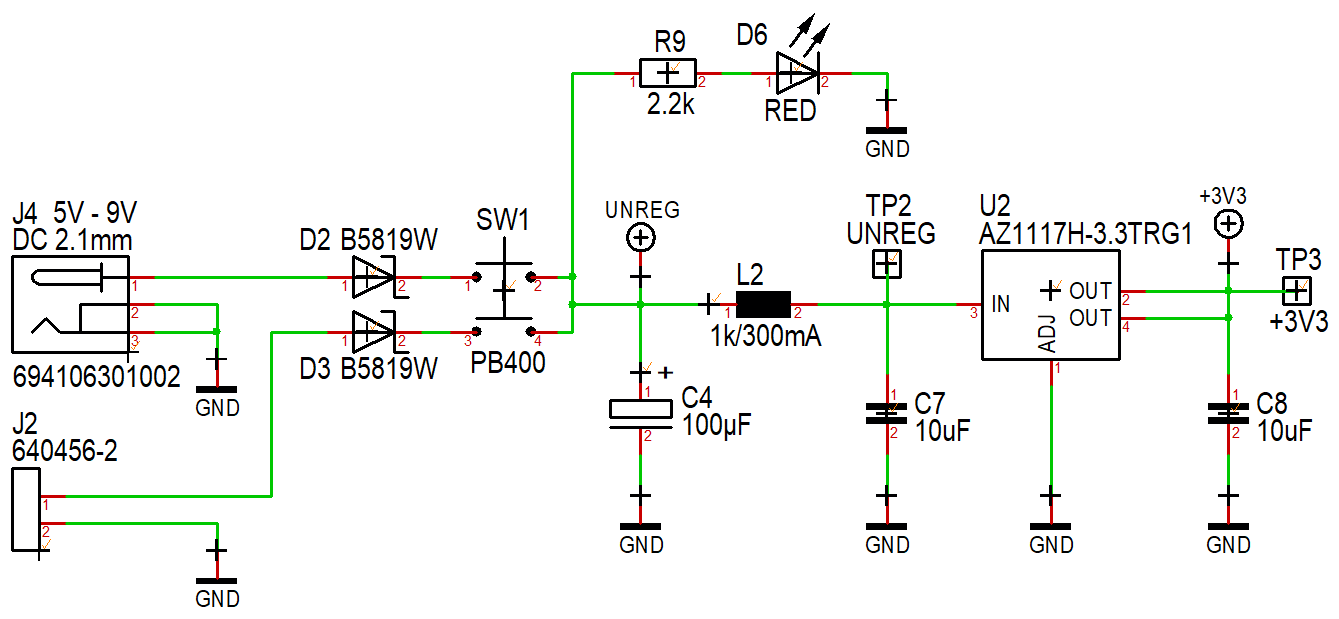
\includegraphics[scale=0.4]{assets/schema-power.png}
\end{center}

\emph{SW1} is the power switch. The diodes \emph{D2} \& \emph{D3} ensure a \textbf{correct voltage polarity,} by letting the current flows only in the right direction. The diodes also select which source (power adapter or battery) powers the \textbf{ZeKit}.

\emph{C4}, \emph{L2} \& \emph{C7} filter the input voltage, \textbf{reducing supply noise.} \emph{U2} regulates down the input, assuring a stable +3V3 in all circumstances. \emph{C8} secures \emph{U2} against possible oscillation of its output voltage.

\subsubsection{Charge Pump}

\begin{center}
    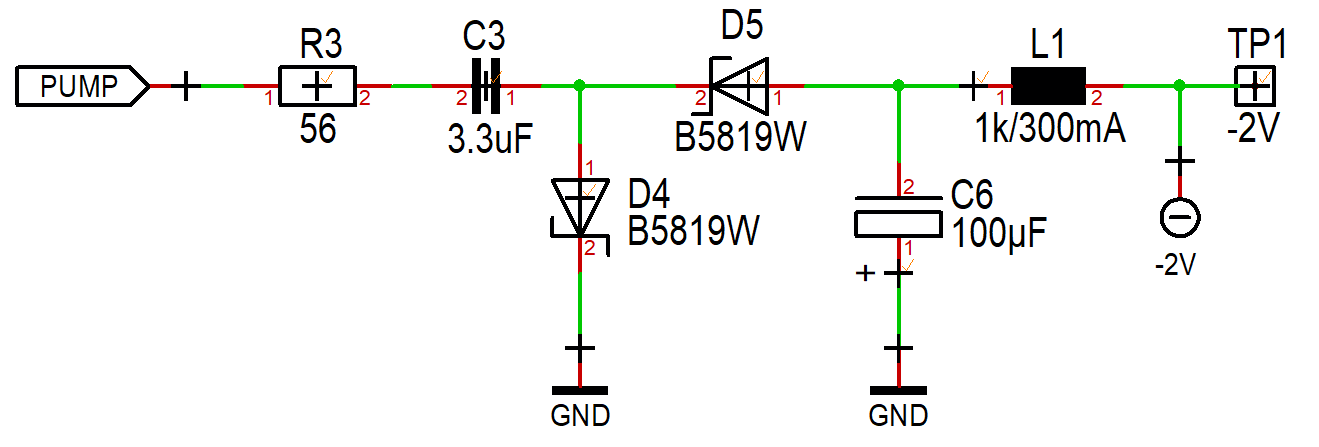
\includegraphics[scale=0.3]{assets/schema-pump.png}
\end{center}

The \emph{PUMP} signal is generated by the MCU and alternates between GND and +3.3V at a high frequency. When \emph{PUMP} is at +3.3V, \emph{C3} is charged via \emph{R3} and \emph{D4}, while \emph{D5} is non-conductive. When \emph{PUMP} is at GND, \emph{D4} is blocking and the charge of \emph{C3} is dumped through \emph{R3}, literally pumping charges from \emph{C6} via the now conducting \emph{D5}.

The inductor \emph{L1} filters the charge pump voltage for better noise immunity.

Ideally, the output voltage at \emph{TP1} would be -3.3V, but because of the losses inside the diodes, it will be around -2V, which is sufficient for proper operation.

\subsection{Microcontroller}

\begin{center}
    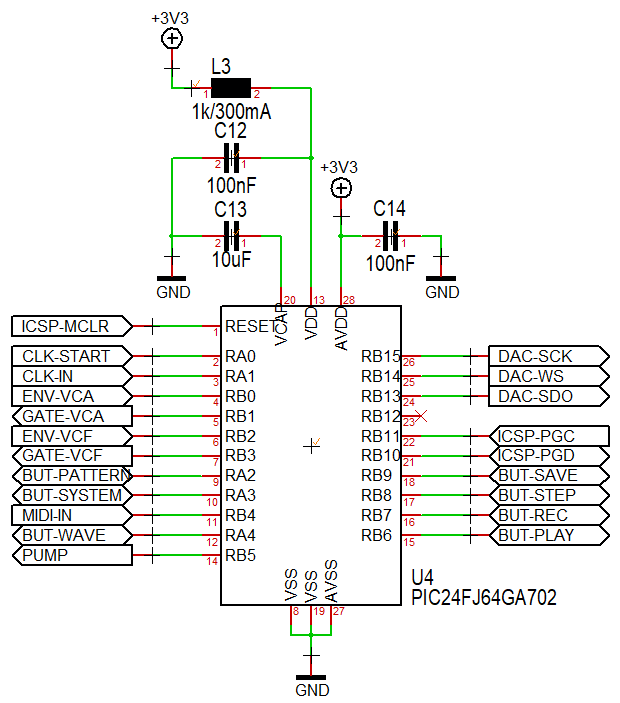
\includegraphics[scale=0.50]{assets/schema-mcu.png}
\end{center}

The \textbf{microcontroller} (MCU) \emph{U4} is the brain of the \textbf{ZeKit}. It processes all signals from the switches and the inputs and generates the \textbf{audio waveforms} as well as control signals for the analog circuitry. This is done by running a firmware that is stored in the internal flash of the chip.

The capacitors \emph{C12}, \emph{C13} and \emph{C14} are used together with the inductor \emph{L3} to improve the stability of the power supply and reduce noise propagation.

\subsection{DAC}

\begin{center}
    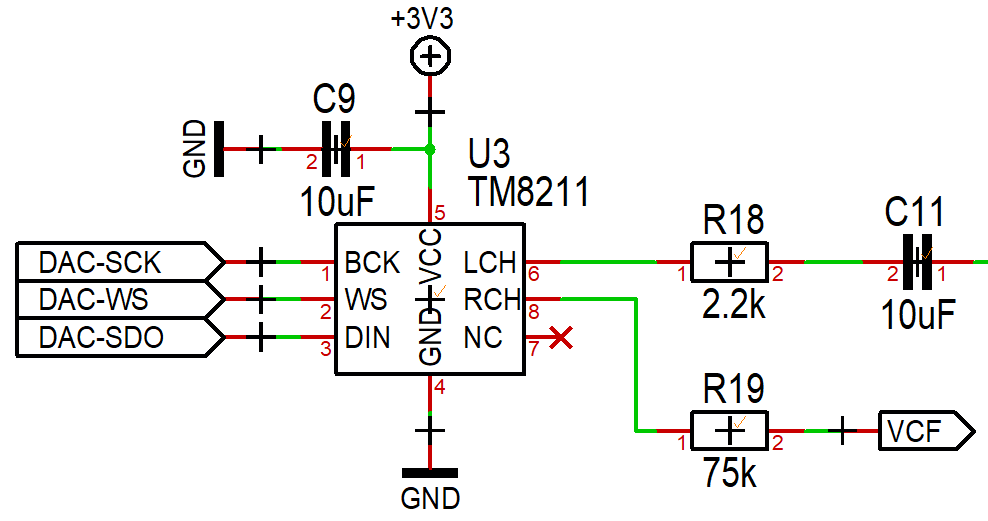
\includegraphics[scale=0.30]{assets/schema-dac.png}
\end{center}

The \textbf{digital-to-analog converter} (DAC) \emph{U3} is directly connected to the MCU via 3 signals. It converts the digital waveforms into a signal in the analog domain. Capacitor \emph{C11} removes the DC offset of the signal, resistor \emph{R18} \& \emph{R19} condition the level to suit the VCF inputs.

This DAC chip provides two independent output channels (audio out and filter cutoff control).

\subsection{VCF}

\begin{center}
    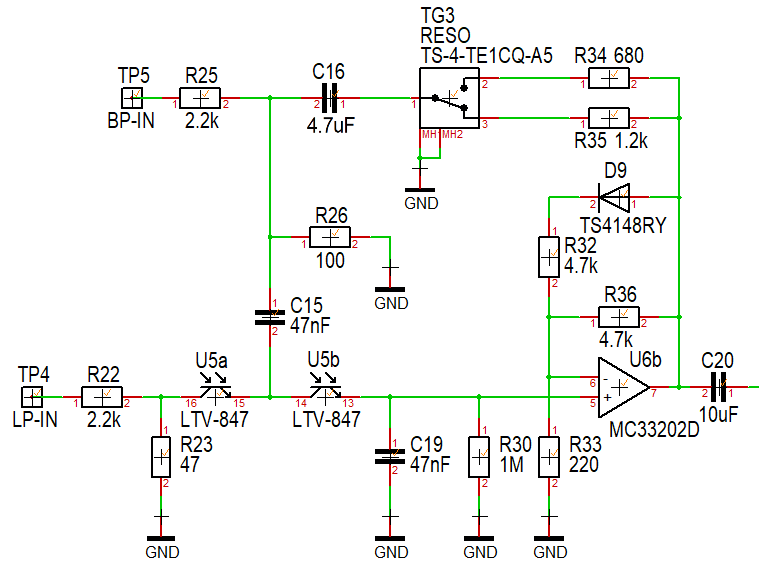
\includegraphics[scale=0.50]{assets/schema-vcf.png}
\end{center}

The filter is a \textbf{2nd order design} with a 12dB/octave slope. The first stage consists of the optocouplers \emph{U5a \& U5b} and the capacitor \emph{C15}, the second stage of the optocoupler \emph{U5b} and the capacitor \emph{C19}. The optocouplers take the role of the resistive elements to control the cutoff frequency.

NOT CHECKED FROM HERE

The input signal \emph{VCF-IN} is decoupled by \emph{C13} and fed in either to the first stage or the feedback path, depending whether low-pass or band-pass configuration is selected by toggle switch \emph{TG1}. The resonance is determined by the feedback loop and can be chosen between two amounts via toggle switch \emph{TG2}. The trimmer \emph{TR2} allows to fine-control one of the settings. The operational amplifier \emph{U6b} provides the necessary gain for driving the next stage and the feedback loop. It utilizes the diode \emph{D7} to tame the amplitude at higher levels by producing a nice-sounding distortion.

\subsection{VCA}

\begin{center}
    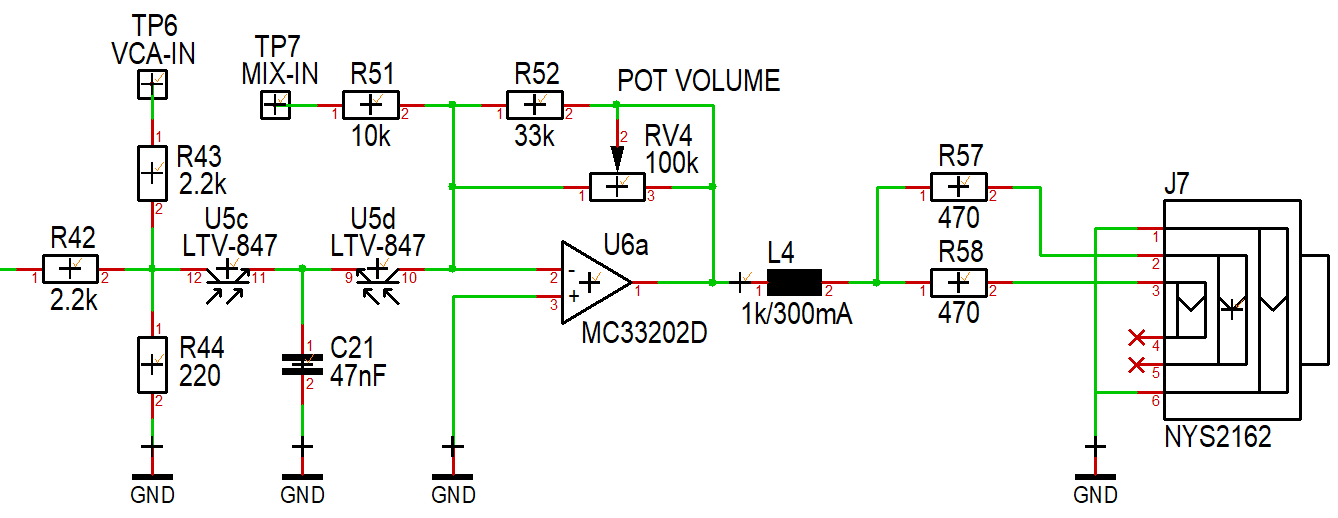
\includegraphics[scale=0.40]{assets/schema-vca.png}
\end{center}

The VCA uses the optocoupler \emph{U3c/U3d} to gain-control the operational amplifier \emph{U6a}. The input signal \emph{VCA-IN} is decoupled by capacitor \emph{C20} and then divided down by resistors \emph{R39} and \emph{R40} to an appropriate level for the optocoupler. To set the output level, the \textbf{Volume} potentiometer is located in the feedback path of the opamp. Resistor \emph{R47} in parallel to the pot provides a nicer control curve for the volume setting. The output is filtered by inductor \emph{L1}, followed by protection resistors \emph{R51} and \emph{R52} and then routed to the output jack \emph{J6}.

\subsection{Envelopes}

\subsubsection{VCF Envelope}

\begin{center}
    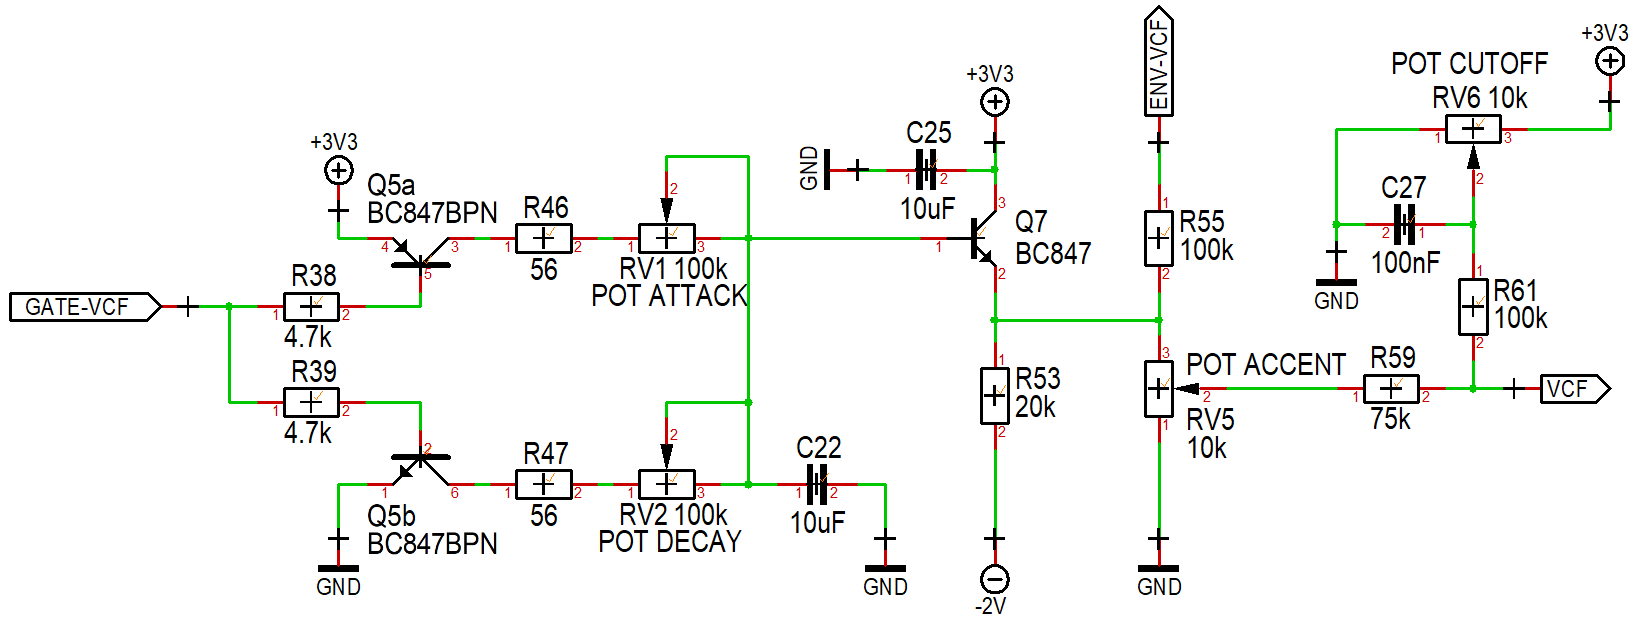
\includegraphics[scale=0.35]{assets/schema-ar-vcf.png}
\end{center}

The filter envelope is generated by either charging capacitor \emph{C23} to +3.3V or discharging it to GND. To start the envelope, the microcontroller sets the \emph{GATE-VCF} signal to +3.3V. The transistor \emph{Q5a} then conducts and \emph{C23} is charged via the resistor \emph{R42} and the \textbf{Attack} potentiometer. To put the envelope in release, the MCU sets the \emph{GATE-VCF} signal to GND. \emph{Q5a} then cuts off and \emph{Q5b} starts to conduct, resulting in \emph{C23} being discharged via \emph{R43} and the \textbf{Release} potentiometer.

The transistor \emph{Q7} acts as a buffer to decouple the envelope. The \emph{ENV-VCF} signal is routed back to the MCU so it can detect that the attack phase is finished. Finally, the envelope amount is set by the \textbf{Accent} potentiometer and added to the constant level set by the \textbf{Cutoff} potentiometer.

\subsubsection{VCA Envelope}

\begin{center}
    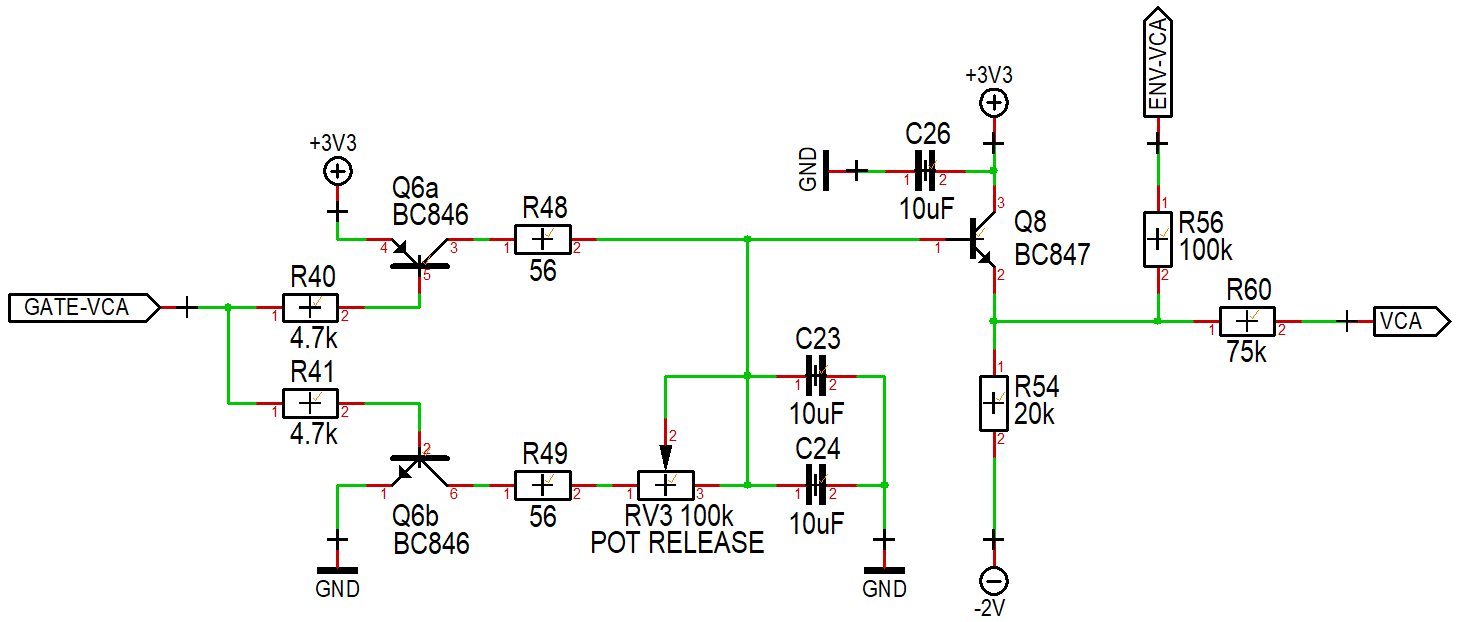
\includegraphics[scale=0.35]{assets/schema-ar-vca.png}
\end{center}

The amplifier envelope works in the same ways as the VCF envelope, but lacks the attack control.

\subsection{Exponential Control Circuit}

\begin{center}
    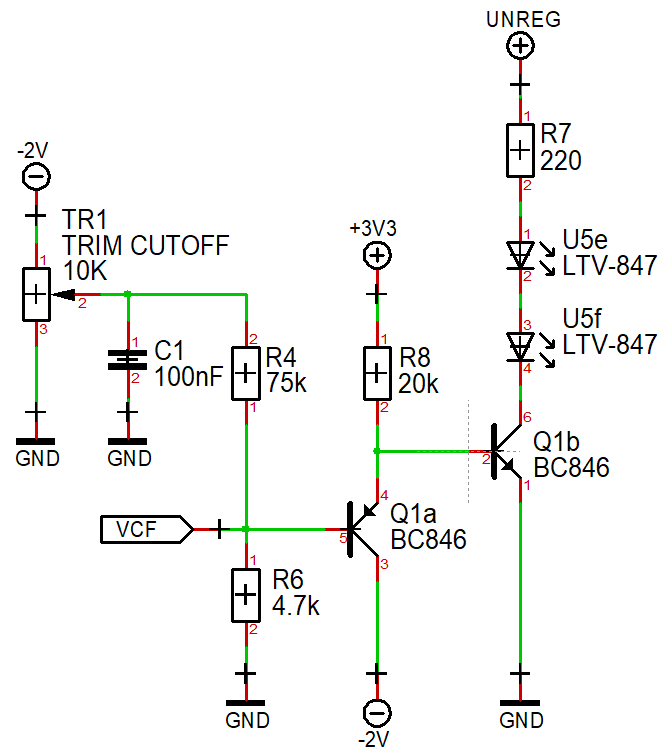
\includegraphics[scale=0.40]{assets/schema-expo-vcf.png}
    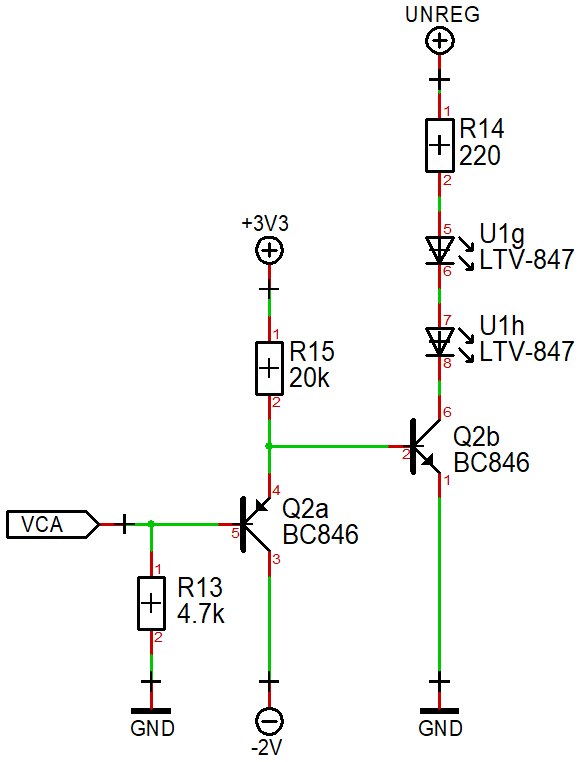
\includegraphics[scale=0.40]{assets/schema-expo-vca.png}
\end{center}

This circuit is used to convert the linear control voltage into an exponential current for the optocouplers. The requirement for this is the nature of our human hearing which recognizes pitches and volumes in an exponential way.

The input of this block uses the signal \emph{VCF} from the filter envelope to drive the buffer transistor \emph{Q1a}. The trim potentiometer \emph{TR1} is used to set a bias level for calibration which is added to the input. The emitter of \emph{Q1a} drives the base of transistor \emph{Q1b} which does the curve conversion. It is based on the fact that the relationship between the base-emitter voltage and the collector current of a transistor is exponential. The collector current of \emph{Q1b} drives the LEDs inside the optocoupler \emph{U5} which controls the filter cutoff.

The VCA uses a similar circuit that is feeded by the VCA envelope.

\subsection{MIDI Input}

\begin{center}
    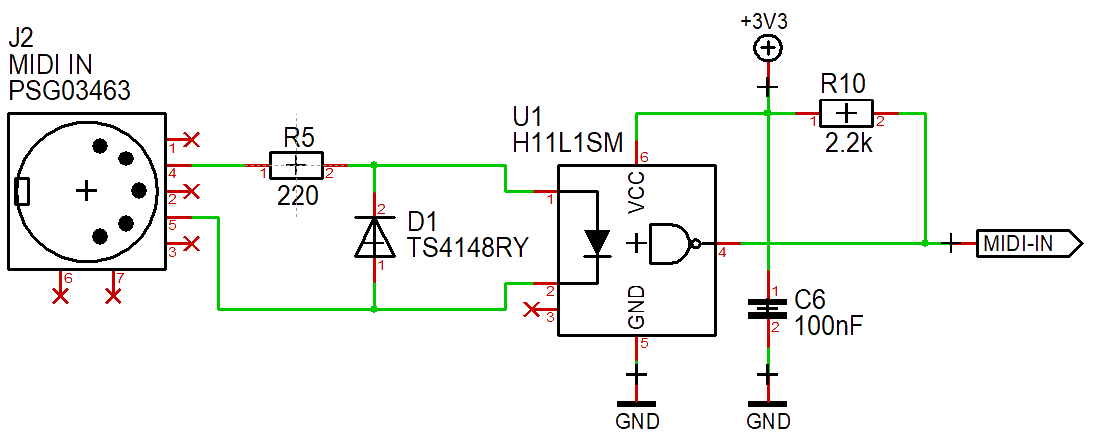
\includegraphics[scale=0.50]{assets/schema-midi.png}
\end{center}

The MIDI input is electrically isolated with an optocoupler to prevent ground loops. This is required by the official MIDI specification. The external device drives the LED inside the optocoupler \emph{U1} via the resistor \emph{R5}. When the LED is on, the photo transistor inside the optocoupler conducts and the \emph{MIDI-IN} signal is pulled to GND. When the LED is off, the photo transistor cuts off and \emph{MIDI-IN} is set to +3.3V by the pullup resistor \emph{R10}.

\subsection{Clock Input}

\begin{center}
    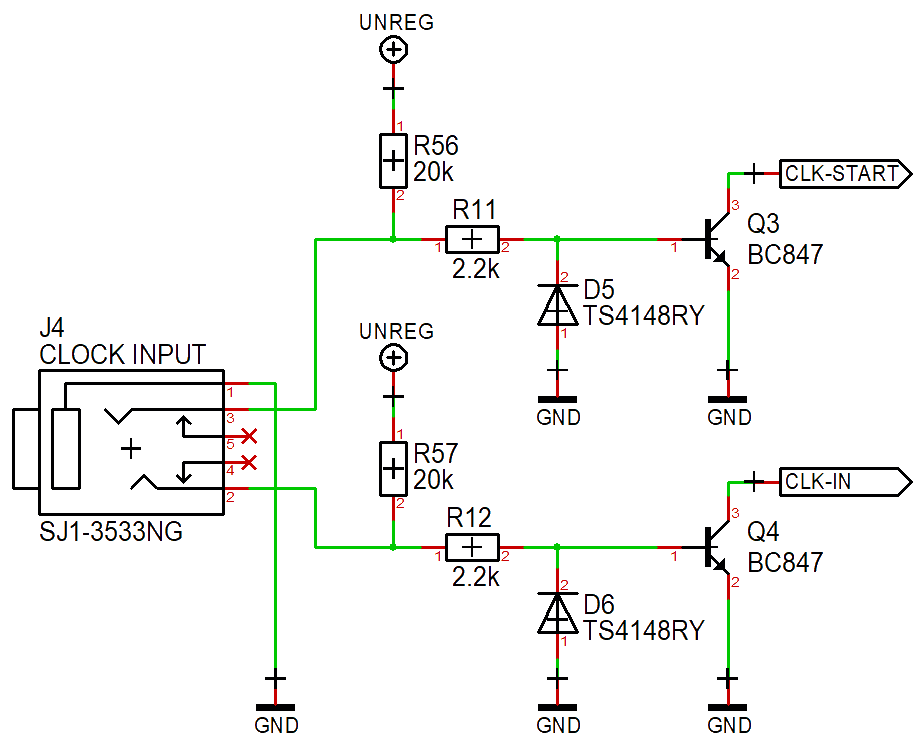
\includegraphics[scale=0.35]{assets/schema-clocks.png}
\end{center}

The clock signal is taken from the tip of the input jack \emph{J4}. If no plug is inserted, a high level is preset by the pullup resistor \emph{R57}. Depending on the input voltage, transistor \emph{Q4} is either conducting or not. Resistor \emph{R12} and diode \emph{D6} protect the transistor against over-voltage or wrong polarity at the input. At the end, the signal \emph{CLK-IN} is then routed to the microcontroller. The MCU uses an internal pullup activated by the firmware to detect the high level when transistor \emph{Q4} is off.

The clock start signal is taken from the ring of the input jack and processed in a similar way by driving the transistor \emph{Q3} to generate the \emph{CLK-START} signal for the MCU.

\subsection{Tactile Switches}

\begin{center}
    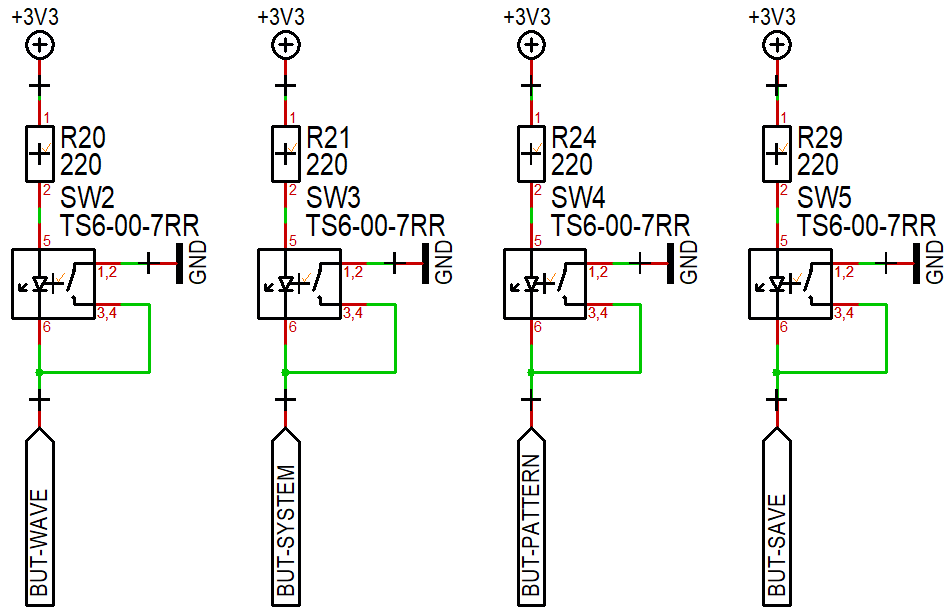
\includegraphics[scale=0.35]{assets/schema-switch.png}
\end{center}

The 7 illuminated tactile switches are directly connected to the microcontroller. The image above shows the \emph{WAVE} button switch \emph{SW2} as an example.

In order to reduce the number of required signal lines, the MCU firmware uses a neat trick: it alternates the mode of the pin connected to the \emph{BUT-WAVE} signal between input and output.

When the MCU pin is configured as input, the button state can be read. In case the button is released, a high level is detected because the pin is connected to +3.3V via the LED and the resistor \emph{R18}. When the button is pressed, the pin is directly connected to GND and a low level is detected. When the MCU pin is configured as output, the LED can be illuminated by driving the signal to GND.

% ------------------------------------------------------------------------------------------
\section{Additional Resources}

\begin{itemize}
    \item GitHub (source code, design files)
    \item Website
\end{itemize}

\pagebreak

% ------------------------------------------------------------------------------------------

\section{Legal Notices}

\textbf{Fred's Lab} cannot be liable for erroneous information contained in this manual. Its contents may be updated without prior notice. We have put our best effort to ensure the information provided here is \textbf{useful and accurate.} \textbf{Fred's Lab} extends no liabilities in regard to this manual other than those required by the local laws.

\vspace{0.25cm}
\begin{center}
    \textbf{Frédéric Meslin Audiogeräte} \\
    Herwarthstraße, 20 \\
    53115 Bonn, Germany \\
    \url{info@fredslab.net} \\
    \url{http://fredslab.net} \\
\end{center}

\vspace{0.25cm}
\textbf{Support requests} \\
For support requests, you can reach us per e-mail at:
\begin{center}
    \url{support@fredslab.net}
\end{center}
or per post, using the company address.

For each support request, please include the \textbf{product model, serial number} and a \textbf{precise description} of the problem encountered with a maximum of details and supporting elements for a quick resolution.

\vspace{0.5cm}
\textbf{Copyright information}

This original manual, its content, including graphics, pictures \& descriptions are the property of \textbf{Fred's Lab}. No part of this manual should be reproduced other than for customer personal use and backup needs without a written permission from \textbf{Fred's Lab}.

\pagebreak

% ------------------------------------------------------------------------------------------
\section{Schematics}
\textbf{Schematics} are provided under the Creative Commons \textbf{CC BY-NC licence}.\\\\
This license allows you to \textbf{remix, adapt, and build upon} this work non-commercially, provided that the derivative works acknowledge the contributions of the original author. 
\vspace{0.25cm}
\begin{center}
    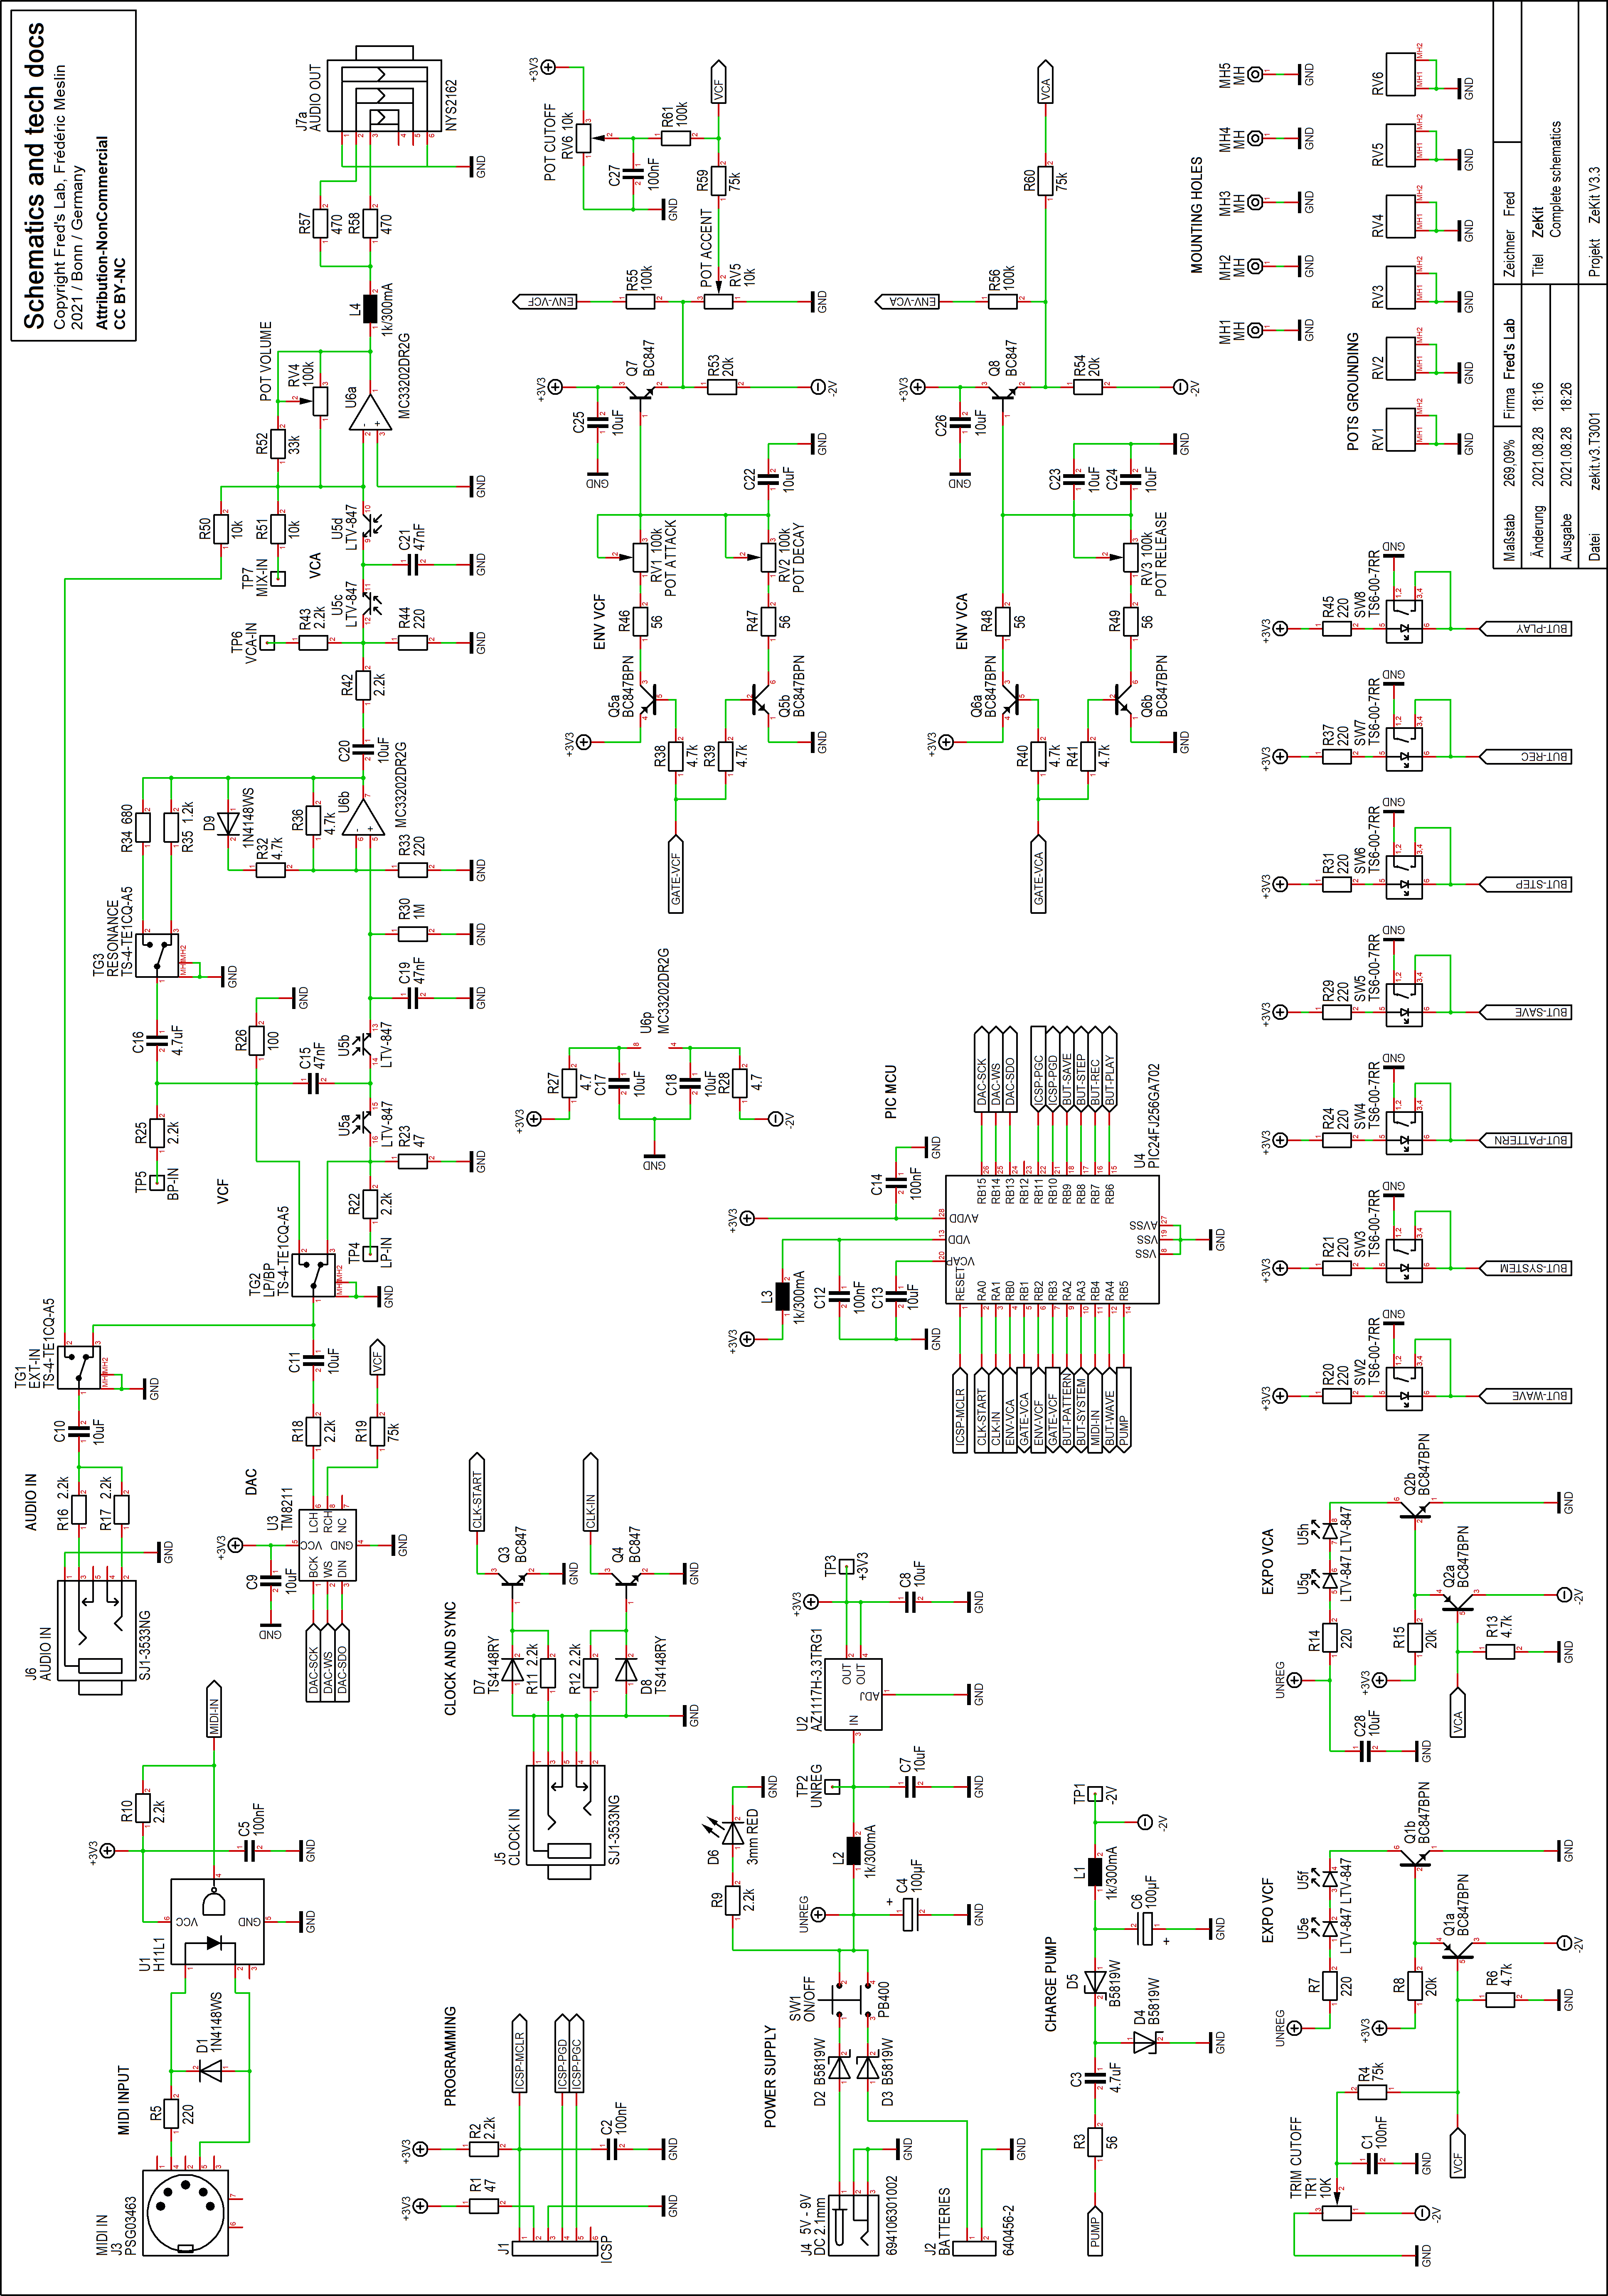
\includegraphics[scale=0.72,origin=c]{assets/schema-full.png}
\end{center}

\section{Bill Of Material}
\vspace{0.25cm}
\begin{center}
    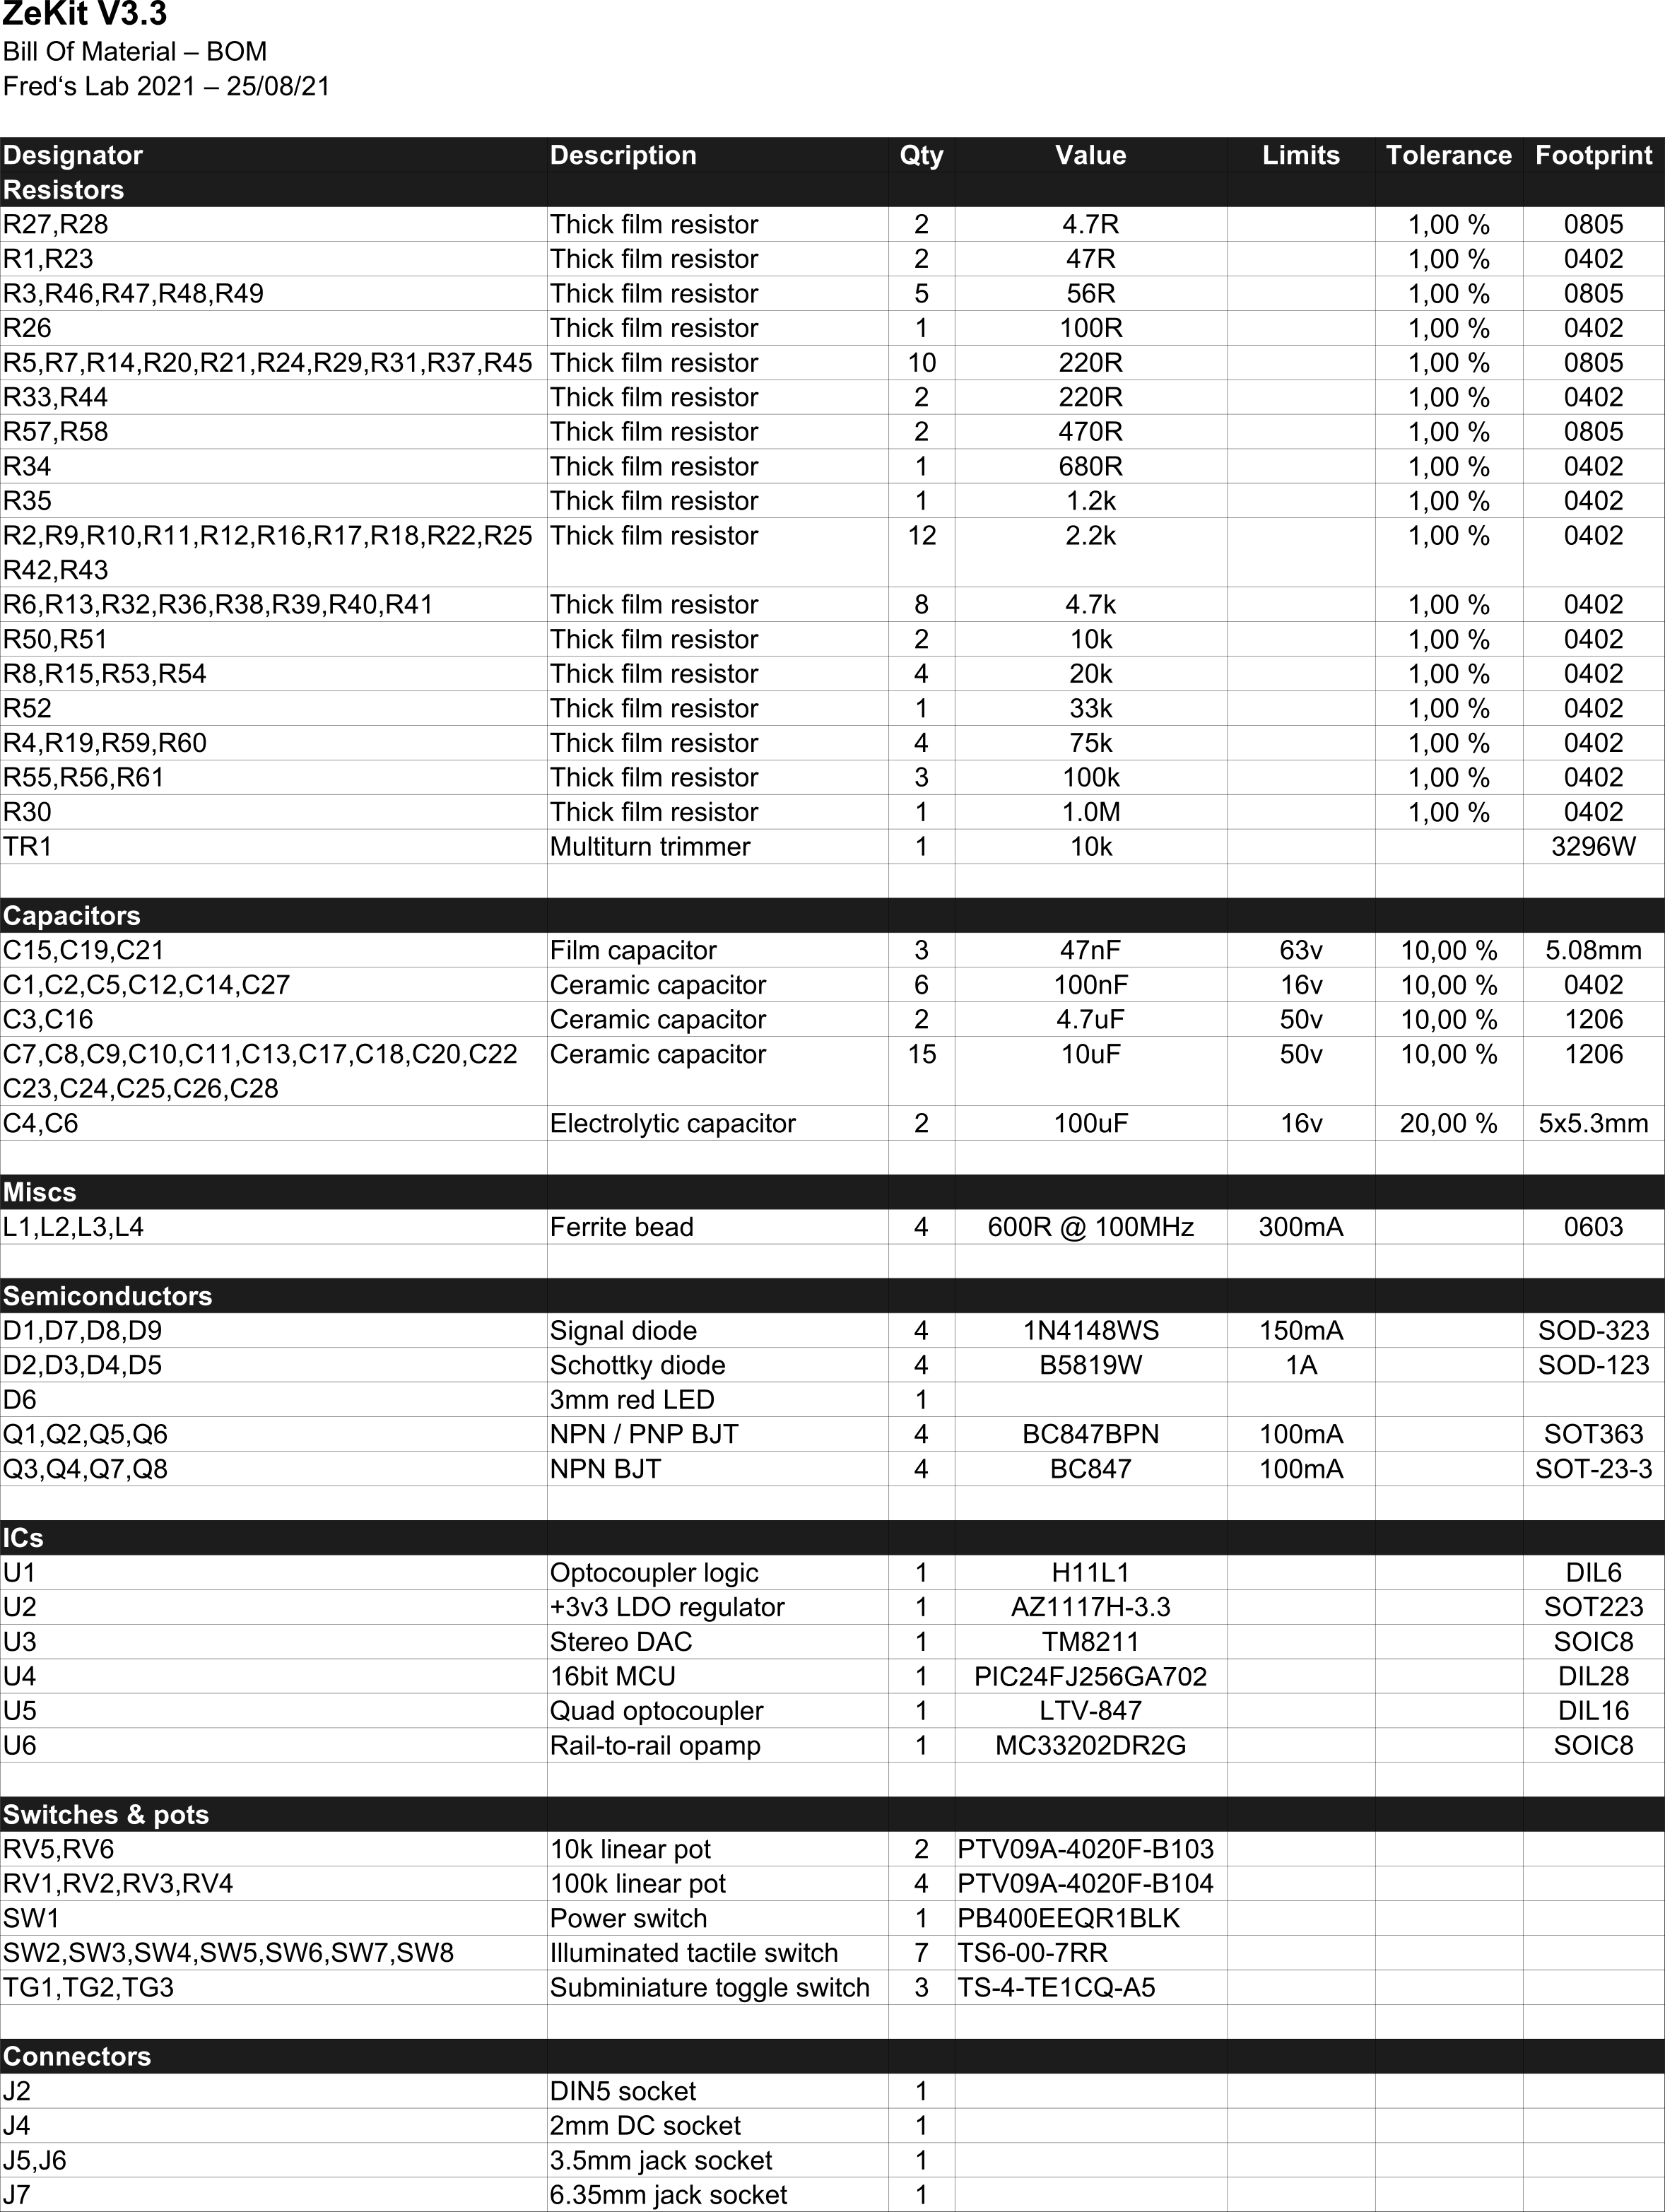
\includegraphics[scale=0.72,origin=c]{assets/bom.png}
\end{center}

\end{document}
